\documentclass[simple,a4paper,14pt,ukrainian,utf8]{eskdtext}

\usepackage[T2A]{fontenc}
\usepackage{amsfonts,amssymb,amsmath,mathtext,cite,float}
\usepackage{setspace}
\usepackage{listings}
\usepackage{indentfirst} % отделять первую строку раздела абзацным отступом тоже
\usepackage[nottoc]{tocbibind}
\usepackage[toc,page]{appendix}
\usepackage{lscape}
\usepackage{lastpage}

\newcommand{\abs}[1]{\lvert#1\rvert} % vector module

\usepackage{geometry} % Меняем поля страницы
\geometry{left=25mm}% левое поле
\geometry{right=1.5cm}% правое поле
\geometry{top=1cm}% верхнее поле
\geometry{bottom=25mm}% нижнее поле

\setcounter{tocdepth}{3}

\renewcommand{\appendixtocname}{Додатки}
\renewcommand{\appendixname}{Додатки}
\renewcommand{\appendixpagename}{Додатки}

\onehalfspacing % полуторный интервал для всего текста
% или \singlespacing % одиночный интервал для всего текста
% или \doublespacing % двойной интервал для всего текста
% или \setstretch{множитель} % произвольный интервал

\DeclareUnicodeCharacter{00A0}{ }

\begin{document}

  \ESKDthisStyle{empty}

  \begin{titlepage}
    \fontsize{10pt}{12pt}\selectfont
    \newpage

    \begin{center}
        Міністерство освіти і науки України \\
        \vspace{1em}
        Житомирський Державний Технологічний Університет \\*
    \end{center}

    \vspace{8em}

    \flushright{Кафедра ПЗС}
    \vspace{1em}
    \flushright{Група ПІ-39М}

    \vspace{8em}

    \begin{center}
        \Large Пояснювальна записка \\ до випускної роботи на тему:
    \end{center}

    \vspace{2.5em}

    \begin{center}
        \Large{\textbf{побудова тривимірної регіональної мапи за допомогою мобільних GPS-пристроїв}}
    \end{center}

    \vspace{6em}

    \begin{flushleft}
        Студент \hrulefill А. Г. Шубович \\

        \vspace{1.5em}

        Керівник роботи \hrulefill А. М. Ковальчук \\

        \vspace{1.5em}

        Завідувач кафедри \hrulefill А. В. Панішев \\
    \end{flushleft}

    \vspace{\fill}

    \begin{center}
        Житомир 2014 р.
    \end{center}

  \end{titlepage}

\newpage

\begingroup
    \ESKDthisStyle{formII}

    \begin{abstract}
        В рамках даної випускної роботи розроблено систему створення тривимірної регіональної мапи за допомогою мобільних GPS-пристроїв. Система складається з двох частин:
        \begin{enumerate}
        	\item \textit{мобільний агент}, котрий зчитує дані з GPS-приймача та/або гіродатчиків і зберігає їх у файл
        	\item \textit{рендерер}, котрий відображає зчитані дані у вигляді тривимірної поверхні та дозволяє переглядати цю поверхню з різних ракурсів
        \end{enumerate}
        
        Було досліджено різні протоколи зберігання даних, зібраних з GPS-приймачів та способи візуалізації гео-даних.
         
        Проект розроблений з використанням мов програмування Java та C++, бібліотеки Qt та платформ Linux та Android.  Мобільний агент працює під керуванням ОС Android. Рендерер може працювати як в оточенні ОС Linux, так і в ОС Windows. Розробка мобільних агентів для спеціалізованих систем наразі триває.

    \vspace{10mm}
    
    \begin{center}
        \textbf{Abstract}    
    \end{center}
    
    	As a part of this work, a complex software system was created. System consists of two main parts:
    	\begin{enumerate}
    		\item \textit{mobile agent}, who reads GPS data and stores it in a file
    		\item \textit{renderer}, who displays the data being read as a three-dimensional surface and allows user to view that surface from different perspectives
    	\end{enumerate}
    	
		Different geo-data storage protocols and geo-data graphic representation methods were inspected as well.
    	
		Project was done using Java and C++ programming languages, Qt libraries, Linux and Android platforms. Mobile agent works under Android OS. Renderer is able to be run under Linux or Windows operating systems. Mobile agents for different task-specific platforms are still being developed.

        \normalsize
        \newpage
    \end{abstract}
\endgroup

\tableofcontents

\newpage

  \clearpage \newpage
  
  \section*{Вступ}
  \addcontentsline{toc}{section}{Вступ}
	
    З нещодавнім масовим впровадженням смартфонів їх використання у повсякденному житті стало нормою для пересічної людини. Область застосування та можливості смартфонів дуже широкі - від читання книжок до тривимірних іграшок та відео-конференцій. Однією дуже корисною функцією сучасних смартфонів є підтримка GPS-навігації. Картографічні та геолокаційні сервіси активно впроваджують соціальну складову. Наприклад, спеціальна організація \textbf{Open Street Map \cite{website:osm}} довірила своїм користувачам редагування мапи світу. Все більш потужними стають і програми навігації, що підтримуються смартфонами і розширюються рамки області застосування цих мобільних пристроїв.

    Не так давно, за допомогою OSM, з’явився термін \textit{маппер}. Це - людина, котра подорожуючи світом, прокладає маршрути та зберігає їх у своєму GPS-пристрої. Після того, як маппер проклав кілька доріг, він завантажує дані на сервери OSM, після чого прокладені ним шляхи з’являються на світовій мапі. І вже за кілька хвилин ці зміни доступні всім користувачам мап OSM.
    
    Немало чим успіх OSM завдячує і розвитку операційної системи Android та смартфонів як популярної мобільної платформи. Завдяки величезній популярності даної ОС, стало можливим поширення мобільних додатків, котрі дозволяють орієнтуватись на місцевості та знаходити шлях до пункту призначення з поточної позиції. Це особливо корисна функція для людей, котрі вперше знаходяться в іншому місті, країні чи просто намагаються знайти певне місце на мапі.
    
    Чимало існує і програм для виконання подібних функцій. Найбільш відомими з них є Яндекс.Карты, Google Maps, OSMAnd, MapWithMe. Але у багатьої випадках, непросто уявити собі вірний маршрут чи обрати більш зручний шлях. Наприклад, у гірській місцевості, шлях між двома точками, який програма вказала як "найкоротший", може зайняти чимало часу через простий факт того, що подібні програми не враховують перепади висот на маршруті. Більшість з таких програм використовують для визначення відстані між двома точками у форматі \textbf{(lat, lng)} \textit{(широта, довгота)} формулу \textbf{Great Circle Distance \cite{website:great_circle_distance}}, яка приймає Землю за ідеальну кулю. Це дає змогу прискорити роботу пошукового алгоритму та зменшити навантаження на процесор, але дає менш точні результати.
    
    Розроблена в рамках даної роботи система чимось нагадує систему OSM та мапперів - мобільні агенти, що запускаються на ОС Android, прокладають шлях на основі даних, зчитаних з вбудованого в смартфон GPS-приймача\cite{website:gps_receiver}. Після цього, маппер передає файл, отриманий в результаті роботи програми, на обробку рендереру, котрий і відображає пройдений маппером шлях у вигляді тривимірної поверхні.
    
    Перегляд маршруту в такому форматі значно поліпшує сприйняття його, дозволяє більш ретельно вивчити всі його складнощі, порівняти з іншими, можливо, більш пологими дорогами.
    
    \textbf{Актуальність теми}
    
    Тема гео-інформаційних систем та навігації набула нового обороту з появою таких пристроїв як смартфони та планшетні ПК. Нині майже кожна людина, опинившись вперше в незнайомому місті, країні або просто вирушивши у похід чи пішу прогулянку природою, може з легкістю знайти маршрут до певного пункту інтересу (Points Of Interest, POI) або до будь-якої іншої точки на мапі просто діставши з кишені смартфон.

	Але задача пошуку та відображення маршруту актуальна не лише для користувачів мобільних та портативних пристроїв. Значна кількість пошукових запитів щодо розташування певного об’єкту чи маршруту між двома точками проводиться і зі звичайних ноутбуків чи стаціонарних комп’ютерів.

	Тому гео-інформаційні та картографічні системи постійно намагаються підвищити комфортність своїх інтерфейсів та інформативність даних, що відображаються.

	Чим більш детально та наближено до реальності буде відображена та чи інша ділянка мапи, тим більша імовірність, що користувач захоче повторити досвід використання даного ресурсу.

	\textbf{Мета та задачі дослідження}
		
	Метою роботи є розробка програмної системи реєстрації та візуалізації геопозиційних даних вздовж множини маршрутів певного регіону з метою створення дорожної мапи регіону.

	Для досягнення вказаної мети треба вирішити наступні основні задачі:
		
	\begin{enumerate}
		\item Провести аналіз наявних технічних засобів отримання даних про поточне розташування, як загально доступних так і комерційних
		\item Розробити програмний засіб для ведення обліку пройденого маршруту
		\item Спроектувати та реалізувати програмний засіб для візуалізації накопичених даних
	\end{enumerate}
	
	\textbf{Об’єктом дослідження} є методи збору та візуалізації даних про трек.

	\textbf{Предметом дослідження} є програмний комплекс, методи та алгоритми збору та візуалізації даних.

	\textbf{Наукова новизна} одержаних результатів полягає у відсутності аналогічного програмного забезпечення на українському ринку зокрема; у зміненні уявлення про гео-інформаційні та картографічні системи.

	\textbf{Практичне значення одержаних результатів}: система активно розробляється та вдосконалюється з метою подальшого введення в експлуатацію науково-дослідницькою лабораторією “Оріон”. 

	Розроблена в межах даної роботи система є лише складовою великого програмно-апаратного комплексу аналізу та візуалізації доріг України. 

	Окремо взятий розроблений у даній роботі компонент може бути застосований як самостійний сервіс користувача для побудови та досконального вивчення маршруту з метою подальшого поширення або пере-використання отриманої інформації.

	\textbf{Структура та обсяг роботи}: атестаційна магістерська робота включає вступ, чотири основні розділи, висновки, список використаних інформаційних джерел та додатки, до яких належать приклади роботи програмної системи. Матеріал атестаційної магістерської роботи викладений на \pageref{LastPage} сторінках. Робота містить ?? рисунків. Бібліографічний список налічує ?? назв.

\clearpage \newpage \section{Технічне завдання}

    Розробити систему збору та відображення гео-позиційних даних про шляхи регіону.

    \begin{enumerate}
        \item Дослідити апаратні можливості платформ з GPS-приймачами
        \item Визначити та проаналізувати наявні формати збереження гео-даних
        \item Порівняти технології побудови та відображення тривимірних фігур
        \item Розробити мобільний агент для ОС Android
        \item Створити рендерер з керованим оглядом поверхні дороги
        \item Провести аналіз та тестування роботи системи в реальному житті
    \end{enumerate}

\clearpage \newpage \section{Постановка задачі та аналіз шляхів її вирішення}

	\subsection{Предметна область}
	
	Розглянуті у даній роботі задачі та побудована для їх вирішення програмна система відноситься більше до \textbf{ГІС \cite{website:gis}}-систем, ніж до прикладних або ж вимірювальних геологічних чи топологічних систем.
	
	Тобто, система призначена для демонстрації, візуалізації та опису географічних об’єктів, а не для їх об’єктивного якісного чи кількісного аналізу.
	
	\subsection{Аналіз існуючих рішень}
	
	Серед наявних програмних засобів існує дві категорії \textit{подібних} до реалізованої в межах даної роботи систем:
	
	\begin{enumerate}
		\item \textbf{гео-інформаційні системи} - системи, за допомогою яких користувач може на мапі знайти той чи інший об’єкт, прокласти маршрут та переглянути інформацію про певні об’єкти
		\item \textbf{системи проектування мапи на кулю} - це поєднання звичайної гео-інформаційної системи та тривимірного інтерфейсу користувача; в системах цього типу мапа не пласка, а накладена у вигляді текстури на кулю
	\end{enumerate}
	
	Реалізована в межах даної роботи програмна система комбінує в собі два цих класи: з одного боку, система дозволяє, як і OSM, вносити зміни до мапи будь-кому, хто має встановлений мобільний агент на свій портативний комп’ютер чи аналогічний пристрій, що містить GPS-приймач; переглядати результати обробки даних від мапперів. З іншого боку, система надає повністю тривимірний інтерфейс користувача - тут мапа не накладається текстурою на певну поверхню, а сама собою являє тривимірну поверхню.
	
	Серед переваг існуючих систем варто відзначити факт наявності орієнтирів та оточуючих об’єктів. Так, користувачам простіше орієнтуватись відносно певних об’єктів. З іншого ж боку, до переваг реалізованої в рамках даної роботи програмної системи, варто віднести більш детальну візуалізацію поверхні Землі, що дає користувачу значно більш точні та наближені до реальності уявлення про місцевість, яку він спостерігає.
	
	\vspace{2em}
	\begin{figure}
		\centering 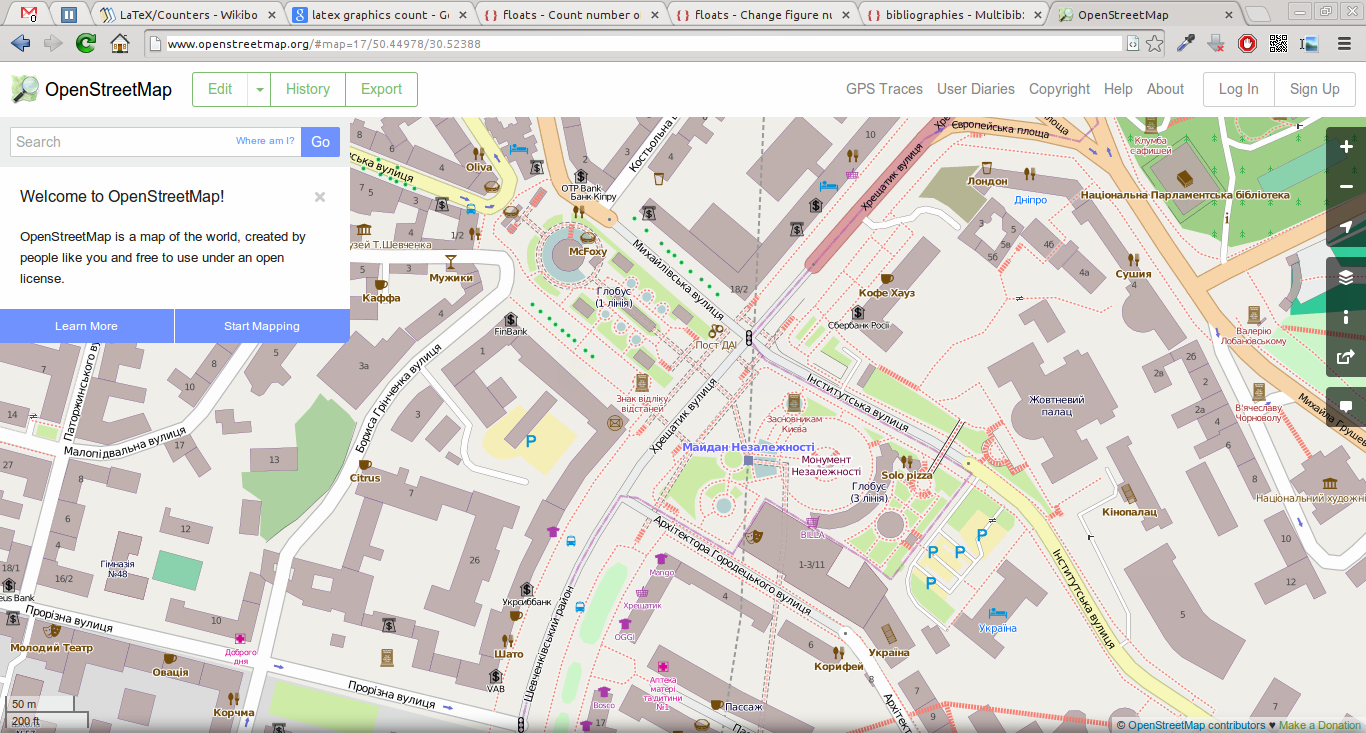
\includegraphics[scale=0.35]{images/osm.png}
		\caption{OpenStreetMap - GIS}
	
		\centering 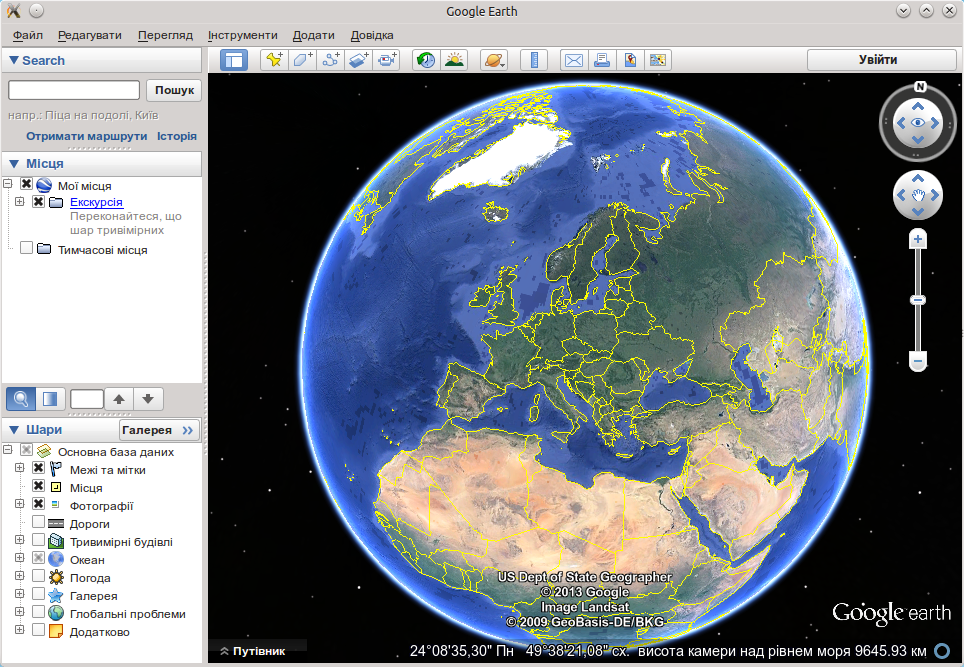
\includegraphics[scale=0.45]{images/google_earth.png}
		\caption{GoogleEarth - система, в якій мапа текстурою накладається на кулю}
	\end{figure}

    \subsection{Пристрої з підтримкою GPS-приймача}
    
    Усі GPS-пристрої поділяються на \textit{професійні} та \textit{приймачі широкого застосування}.
	
	Професійні GPS-приймачі можна розділити на дві категорії:
    
    \begin{enumerate}
    	\item \textbf{геодезичні приймачі} - пристрої для геодезичних робіт у польових умовах
    	\item \textbf{приймачі ГІС-класу} - такі собі кишенькові портативні комп’ютери з вмонтованим GPS-приймачем
    \end{enumerate}
    
    GPS-приймачі для широкої цільової аудиторії поділяються на два види пристроїв навігації:
    
    \begin{enumerate}
    	\item \textbf{GPS-навігатори}, основна функція котрих - прийом та обробка сигналу гео-позиціювання зі супутників
    	\item \textbf{пристрої, що містять GPS-приймач}, де навігація та гео-локація не є основними цілями використання цих пристроїв
    \end{enumerate}
    
    Пристрої відрізняються якістю виготовлення компонентів (особливо антенн), програмним забезпеченням, режимами роботи, робочими діапазонами частот, алгоритмами подавлення інтерференційних залежностей, сонячної активності, системами навігації, терміном роботи від одного заряду акумулятора та, звісно ж, вартістю.

    Логічно було б припустити, що в якості платформи для мобільних агентів краще використати саме GPS-навігатори. Але моделей їх існує безліч, кожна з яких має свої особливості та інструментарій для розробки. 
    
    З іншого ж боку, моделей смартфонів на основі ОС Android чи iOS з вбудованим GPS-приймачем хоч і багато, зате особливості роботи та інструментарій для розробників у таких пристроїв стандартизовані. До того ж, вони значно більш поширені серед звичайних людей.
    
    Саме тому з метою збільшення цільової аудиторії мапперів було вирішено взяти за основу смартфони під керуванням ОС Android.

    \subsection{Формати GPS-даних}
    
    В якості формату спілкування GPS-приймача та різноманітних засобів обробки гео-даних (як програмних так і апаратних) використовуються варіації стандарту NMEA (\textit{National Marine Electronics Association}).
    
    Існує дві основних версії цього стандарту:
    
    \begin{enumerate}
    	\item \textbf{NMEA 0183 \cite{website:nmea_0183}}, який використовується у більшості не спеціалізованих програмних та апаратних засобів
    	\item \textbf{NMEA 2000 \cite{website:nmea_2000}}, який використовується у мережі подібних між собою пристроїв у морській та залізничній інфраструктурах
    \end{enumerate}
    
    Дані у форматі NMEA - це послідовність спеціальним чином відформатованих рядків. Стандат NMEA описує багато різних  форматів даних. Серед них:
    
    \begin{enumerate}
    	\item \textbf{AAM} - час до пункту призначення
        \item \textbf{ALM} - дані альманаху
        \item \textbf{APA} - рядок "А" авто-пілоту
        \item \textbf{APB} - рядок "В" авто-пілоту
        \item \textbf{BOD} - напрямок від точки відліку до точки призначення
        \item \textbf{BWC} - напрямок з використанням формули Great Circle
        \item \textbf{DTM} - використана дата
        \item \textbf{GGA} - дані про старт GPS-модуля
        \item \textbf{GLL} - дані про широту/довготу
        \item \textbf{GSA} - загальна інформація про супутники
        \item \textbf{GST} - проміжок шумів
        \item \textbf{GSV} - детальна інформація про супутники
        \item \textbf{RMB} - рекомендований інформаційний рядок даних GPS
        \item \textbf{RMC} - рекомендований короткий рядок даних GPS
        \item \textbf{RTE} - повідомлення про маршрут
        \item \textbf{VBW} - морська швидкість
        \item \textbf{VTG} - напрямок вектору швидкості над землею
        \item \textbf{WCV} - швидкість наближення до чергової проміжної точки
        \item \textbf{WPL} - інформація про розташування чергової проміжної точки
        \item \textbf{ZDA} - дата та час
    \end{enumerate}
    
    Кожен рядок даних у форматі NMEA 0183 має наступний вигляд:
    
    \begin{enumerate}
    	\item \textbf{символ \$}
		\item \textbf{ідентифікатор повідомлення} - дві літери, що визначають джерело сигналу та три літери, що визначають вміст рядка (тип даних)
		\item \textbf{дані} - список полів, розділених комами
		\item \textbf{CRLF} - кінець рядка
    \end{enumerate}
    
    Так, в полі даних у форматі RMC зберігаються:
    
    \begin{enumerate}
    	\item \textbf{дата та час отримання позиції від супутника}
    	\item \textbf{широта та довгота}
    	\item \textbf{точка відліку широти та довготи} - вказує, з якого меридіану починається відлік широти та довготи: північ чи південь, захід чи схід
    	\item \textbf{прапорець валідації} - вказує чи корректні надіслані супутником дані
    \end{enumerate}
    
    В даній роботі було використано два типи рядків - \textbf{GPRMC} (Recommended Minimum sentence C), дані про поточне гео-розташування приймача та \textbf{PGRMZ} - дані про поточну висоту над рівнем моря у поточному гео-розташуванні приймача. Цих даних достатньо для побудови цілком відповідної реальності тривимірної поверхні пройденого шляху.

	\subsection{Проблеми при рішенні поставленої задачі}
	
	Перша проблема, з якою довелось зустрітись на початку процесу розробки системи полягає у тому факті, що GPS-модуль ОС Android хоч і описує та використовує подію під назвою \textit{locationChanged} ("гео-позиція змінилась"), але не сприймає зміну позиції як зміну координат чи висоти над рівнем моря. Натомість ця подія означає прийнятий від супутника мережі GPS сигнал, котрий містить дані про поточне положення. 
	
	Це спричиняє надмірні дубльовані дані, що збільшує обсяги даних, котрі зберігаються на такому доволі непотужному пристрої як смартфон чи планшетний ПК. 
	
	Для усунення цієї проблеми було створено двоетапну фільтрацію даних на предмет наявності дубльованих даних про положення. Слід відмітити, що фільтруються лише друге та подальші входження одного і того ж запису, але лише за умови що \textbf{ці дані слідують підряд один за одним}.
	
	Найбільш значна та складна в усуненні проблема, яка виникла вже на останніх етапах розробки системи, під час тестування - неточності та похибки у отриманих GPS-даних.
	
	Так, скажімо, якщо мобільний агент працює на смартфоні, котрий лежить в кишені маппера, то сигнал буде дуже сильно вар’юватись так як людина при ходьбі чи їзді на велосипеді здійснює різні рухи, що спричиняє зміщення пристрою в кишені. А це, у свою чергу, призводить до прийому хибних даних про висоту чи гео-позицію:
	
	\vspace{2em}
	\begin{figure}
		\centering 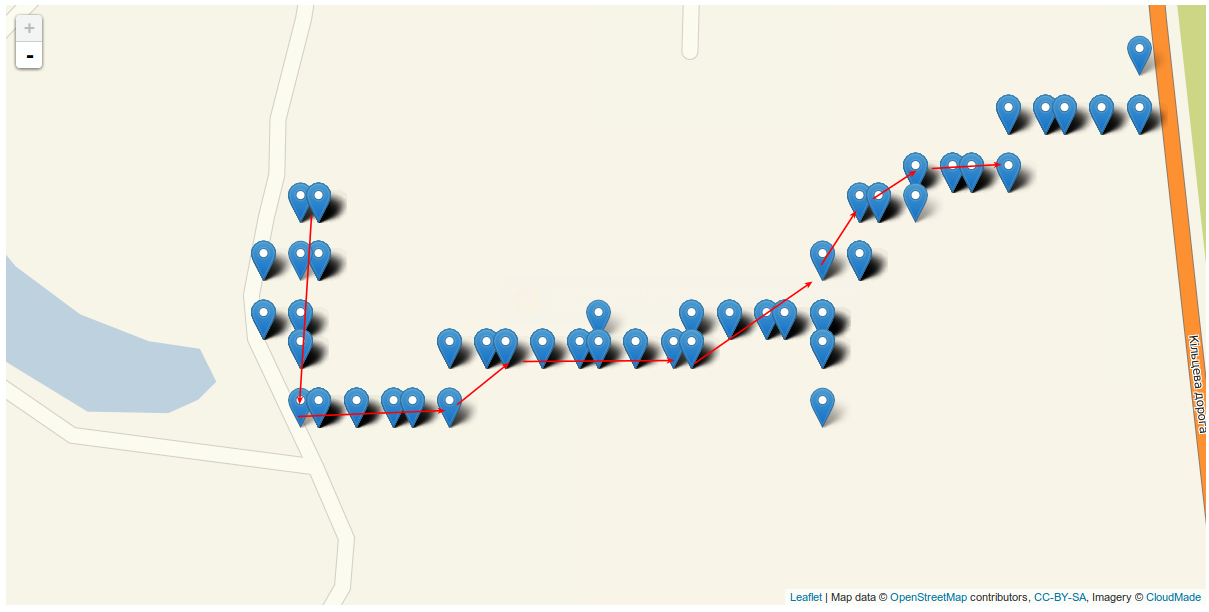
\includegraphics[scale=0.35]{images/errors1.png}
		\caption{Похибки GPS-сигналу; стрілками показано пройдений маршрут}
	\end{figure}

	\vspace{2em}
	\begin{figure}
		\centering 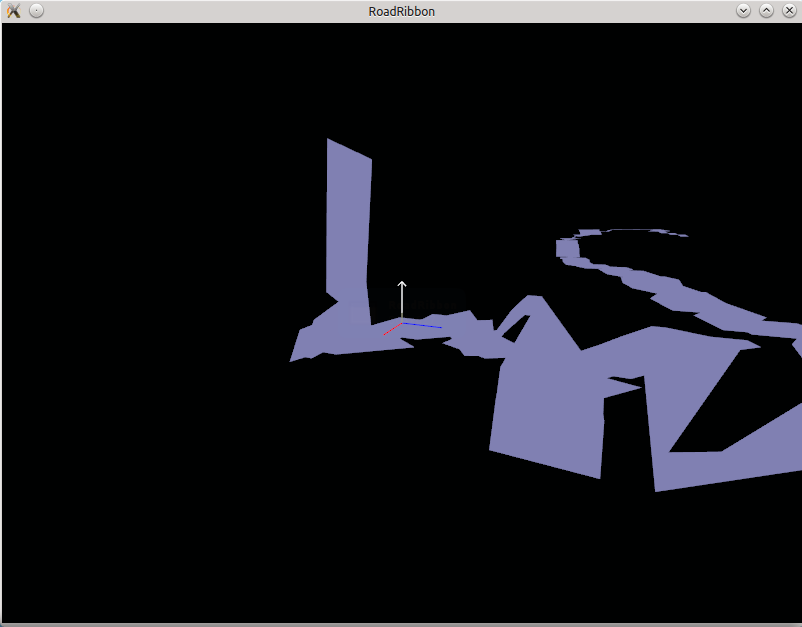
\includegraphics[scale=0.5]{images/errors2.png}
		\caption{Похибки GPS-сигналу під час візуалізації}
	\end{figure}
	
	З іншого ж боку, якщо мобільний агент працює на пристрої, що знаходиться у автомобілі, під час руху останнього похибок буде значно менше, так як рух автомобіля більш амортизований завдяки підвісці та рессорам.
	
	На сигнал супутників мережі GPS також впливають такі чинники, як
	
	\begin{enumerate}
		\item \textbf{якість антенни модуля GPS} - дешеві або погано виконані компоненти GPS-приймача, а особливо - антенна, багато в чому визначають якість прийому сигналу супутників
		\item \textbf{ясність неба} - атмосферні ефекти сповільнюють радіо-сигнал супутників, через що сигнал від супутника може надійти з затримкою і, відповідно, міститиме дані про вже неактуальне положення
		\item \textbf{кількість супутників у видимій обмеженій частині небесної сфери} - дані від одного супутника можуть бути хибними; тому більшість виробників GPS-приймачів передбачають апроксимацію у визначенні положення, опираючись на дані кількох (зазвичай 5 .. 12) супутників
		\item \textbf{кількість об’єктів довкола приймача}	 - сигнал супутників постійно відбивається від різних об’єктів, що знаходяться довкола приймача. Тому чим менше таких об’єктів - тим більш "чистим" буде отриманий сигнал
		\item \textbf{актуальність даних про орбіти супутників} - орбіти супутників періодично змінюються, тому для корегування отриманого сигналу дані про орбіти супутників на приймачі потрібно час від часу оновлювати
	\end{enumerate}
	
	Сумарна похибка може сягати $\pm 15$ метрів. Через це може виникати багато артефактів, помітних лише на етапі візуалізації треку.
	
	Одне з можливих рішень даної проблеми - використання даних від інших датчиків, як, наприклад, акселерометри. Але такий алгоритм можна застосовувати лише за умови відсутності шумових зміщень GPS-приймача. Що вже відкидає можливість застосування цього методу для мапперів, що пересуваються пішки або на велосипедах.
	
    \subsection{Відтворення шляху на мапі}
    
    З метою перевірки роботи алгоритму дешифрування даних, записаних мобільним агентом, було створено HTML-сторінку, за допомогою якої можна перевірити достовірність та точність даних.
    
    Сторінка використовує бібліотеку \textbf{leaflet} для керування відображенням мапи та маркерів на мапі. Для дешифрації рядків даних у форматі NMEA-0183, отриманих під час роботи мобільного агента, використовується невеликий скрипт мовою програмування \textbf{JavaScript}.
    
    У браузері набір даних, зібраних за допомогою спеціально облаштованого транспортного засобу, виглядає так:
    
    \vspace{3em}
    \begin{figure}
	    \centering 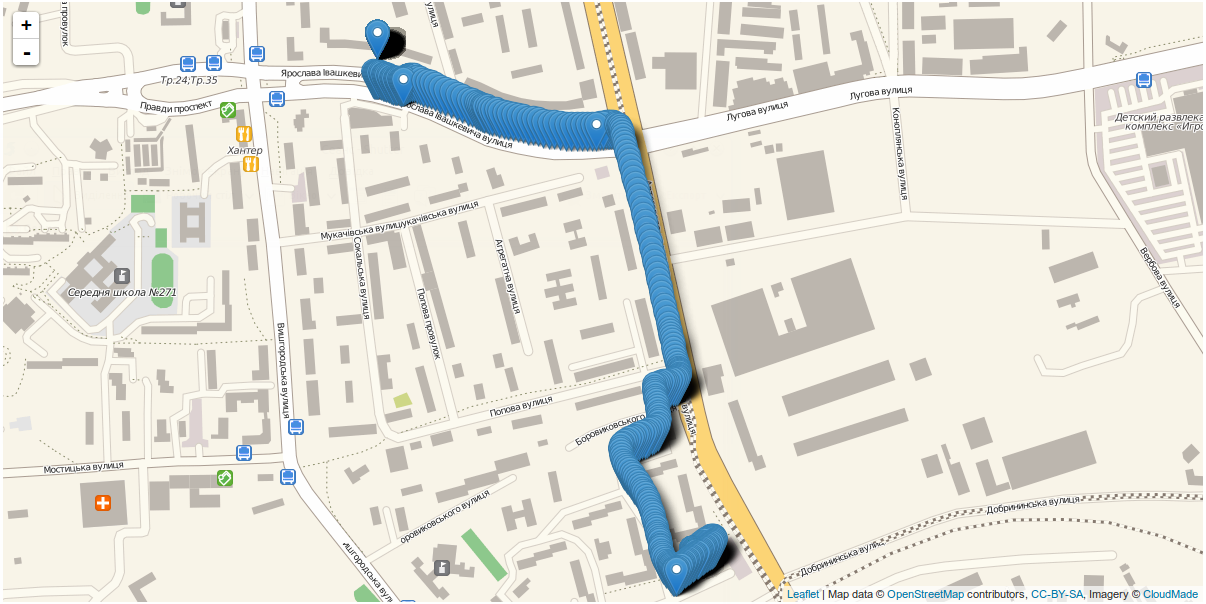
\includegraphics[scale=0.34]{images/leaflet_renderer.png}
	    \caption{Візуалізація треку на мапі}
	\end{figure}
    
    \newpage
    	
    \subsection{Відтворення шляху у вигляді двовимірного кістяка}
    
    Однією з перших поставлених цілей реалізації рендерера стояла реалізація алгоритму побудови двовимірного зображення пройденого маршруту, або ж його кістяка. 
    
    \textit{Кістяк маршруту} - це набір опорних точок чи ліній, на основі яких згодом будується пласка або тривимірна поверхня.
    
    Побудувавши плаский кістяк шляху у тривимірному просторі, можна вдосконалити його, піднявши ключові лінії на необхідну висоту та з’єднавши їх між собою поверхнями.
    
    З цією метою було сповна використано можливості графічного модуля бібліотеки \textbf{SFML}.
    
    \vspace{3em}  
    \begin{figure}  
	    \centering 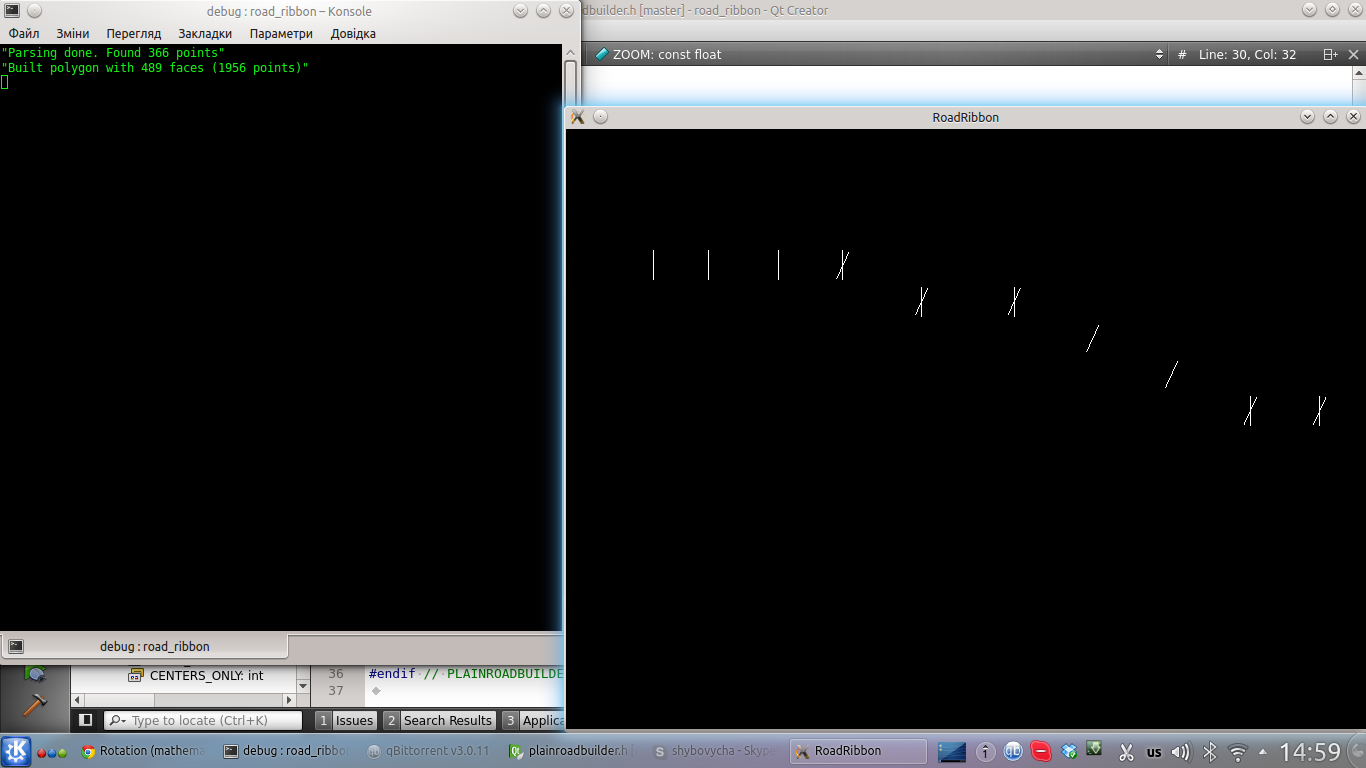
\includegraphics[scale=0.34]{images/road2d_2.png}
	    \caption{Двовимірний кістяк треку}
	\end{figure}
    
    \subsection{Побудова тривимірної поверхні}
    
    Для побудови тривимірної поверхні треку використовується один з двох підходів:
    
    \begin{enumerate}
    	\item \textbf{обробка даних гіродатчиків} - якщо інша опція недоступна
    	\item \textbf{обробка даних GPS} - використовуються зчитані дані про висоту над рівнем моря
    \end{enumerate}
    
    Якщо GPS-приймач на пристрої має змогу отримувати дані про висоту над рівнем моря в поточній позиції, ці дані будуть використані для побудови тривимірної поверхні треку. Так як дані цього типу не потребують додаткової обробки, даний метод найбільш приорітетний.
    
    Якщо ж GPS-приймач не надає можливості використовувати дані про висоту над рівнем моря, тоді мобільний агент перевіряє, чи доступний для використання так званий \textbf{G-серсор}. Якщо це вірно, то використовуються дані про поточний нахил GPS-приймача або смартфону та відстань до попереднього розташування (з використанням формули \textit{Great Circle Distance}) для отримання значення висоти, використовуючи властивості тригонометричних функцій.
    
    \subsection{Зміна перспективи огляду поверхні у просторі}
    
    Оскільки тривимірна поверхня треку в чистому вигляді (без фонових декорацій накшталт небесної сфери, ландшафту, предметів та будівель оточення, тощо) не дуже зручна для використання, було створено примітивний вказівник напрямків основних векторів тривимірного простору та додано орбітальну камеру, котра обертається довкола цього вказівника.
    
    Для зручного перегляду тривимірної поверхні дороги, камеру можна пересувати у восьми напрямках - вперед/назад, вгору/вниз та ліворуч/праворуч. Всі переміщення здійснюються відносно поточного розташування центру обертання камери - вказівника напрямних векторів простору.
    
    Обертання камери довкола центру обертання реалізовано за допомогою алгоритму множення кватерніонів.
    
    У поточній програмній реалізації рендерера це виглядає ось так:
    
    \vspace{3em}
    \begin{figure}
	    \centering 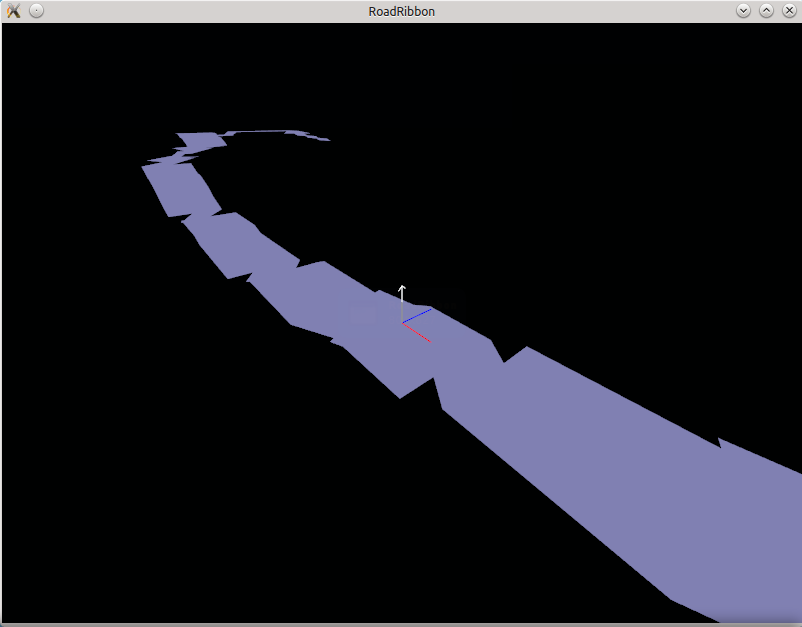
\includegraphics[scale=0.5]{images/camera1.png}
	    \caption{Огляд візуалізації за допомогою орбітальної камери}
	\end{figure}
    
\clearpage \newpage \section{Проектування системи}

    \subsection{Вибір інструментальних засобів}

        В якості мови програмування для створення мобільного агенту було обрано Java, так як

        \begin{itemize}
            \item мова містить лише необхідні та достатні для розробки конструкції
            \item мова компільована
            \item код мовою Java для розв’язку конкретно даної задачі виходить лаконічним та гнучким
            \item має чудову підтримку спільноти та гарну документацію - швидке вирішення більшості проблем за їх вникнення
            \item низький поріг входження - швидкий старт роботи з мовою програмування
            \item велика кількість готових рішень, написаного коду та бібліотек
        \end{itemize}
        
        Для створення рендерера було обрано мову програмування C++ за необхідності роботи з великими обсягами даних та тривимірним малюванням. 
        
        Для спрощення роботи було використано бібліотеки платформи Qt. Це дозволило спростити роботу з рядками, регулярними виразами та деякими контейнерними структурами даних.
        
        В якості бібліотеки для побудови та відображення двовимірної та тривимірної поверхні дороги було обрано OpenGL. Ця графічна система дозволяє просто та водночас ефективно працювати з двовимірними та тривимірними зображеннями та об’єктами. Поріг входження в цю систему значно нижчий за, скажімо, DirectX. А той факт, що система платформонезалежна дає змогу реалізувати рендерер для різних користувачів.
        
        З іншого ж боку, існуючі графічні чи ігрові двигунці та бібліотеки мають значно простіший інтерфейс для реалізації тих чи інших задач. Усі вони являють собою вищий рівень абстракції, ніж OpenGL чи DirectX. Але усі вони значно "важчі" для рішення задач подібного об’єму.
        
        Для створення контексту роботи OpenGL, обробки подій введення, створення та обробки зображень було використано бібліотеку SFML. Функціональні можливості цієї бібліотеки значно ширші за SDL, GLUT та інші, а програмний інтерфейс - простіший.
        
        Для розробки мовою С++ було використано інтегроване середовище розробки (IDE) \textbf{QtCreator}. Основною причиною того є зручний користувацький інтерфейс та підтримка платформи Qt "з коробки".
        
        \vspace{2em}
        \begin{figure}
        	\centering 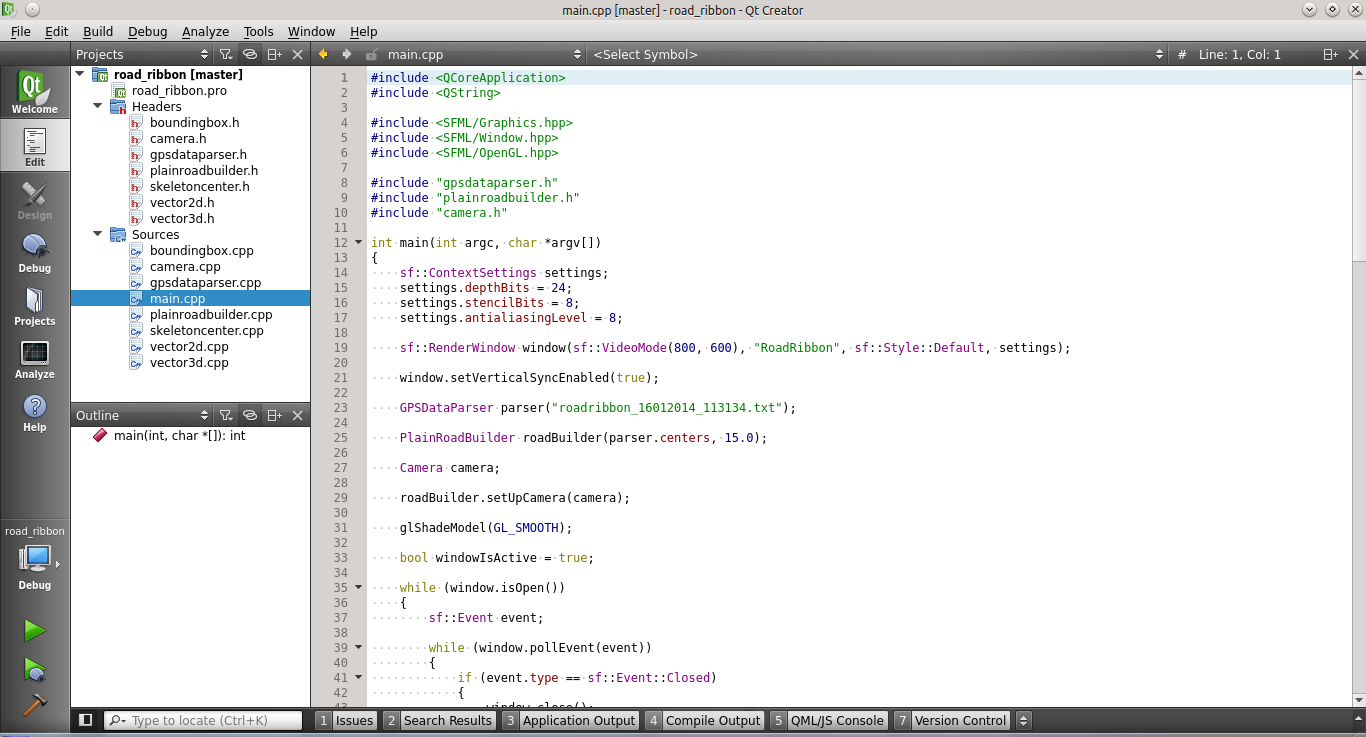
\includegraphics[scale=0.35]{images/qt_creator.png}
        	\caption{IDE QtCreator}
        \end{figure}
        
        Для розробки під платформу Android використовувалось середовище розробки AndroidStudio. Це середовище є модифікацією IntelliJ Idea Community Edition, що дає такі вагомі переваги над іншими аналогами, як:
        
        \begin{enumerate}
        	\item \textbf{"розумне" авто-доповнення коду} - середовище має потужний лексичний аналізатор коду, який дуже точно підказує, що програміст мав на увазі, коли в даному блоці коду почав вводити даний текст; на відміну від більшості редакторів, які просто підказують будь-які можливі фрази, які починаються з введених програмістом символів
        	\item \textbf{"розумний" пошук та заміна} - завдяки функції індексації вихідного коду проекту, середовище розробки знаходить всі можливі (статичні та динамічні використання) введеної фрази
        	\item \textbf{підтверджені розробниками плагіни} - плагіни до середовищ розробки, заснованих на IntelliJ Idea ретельно перевіряються розробниками, що виключає більшість недоліків у самих плагінах
        	\item \textbf{зручний графічний інтерфейс} - інтерфейс побудований таким чином, щоб програміст максимально сконцентрувався на коді, який він пише, а не на можливостях середовища, в якому він пише код
        \end{enumerate}
        
        \begin{figure}
        	\centering 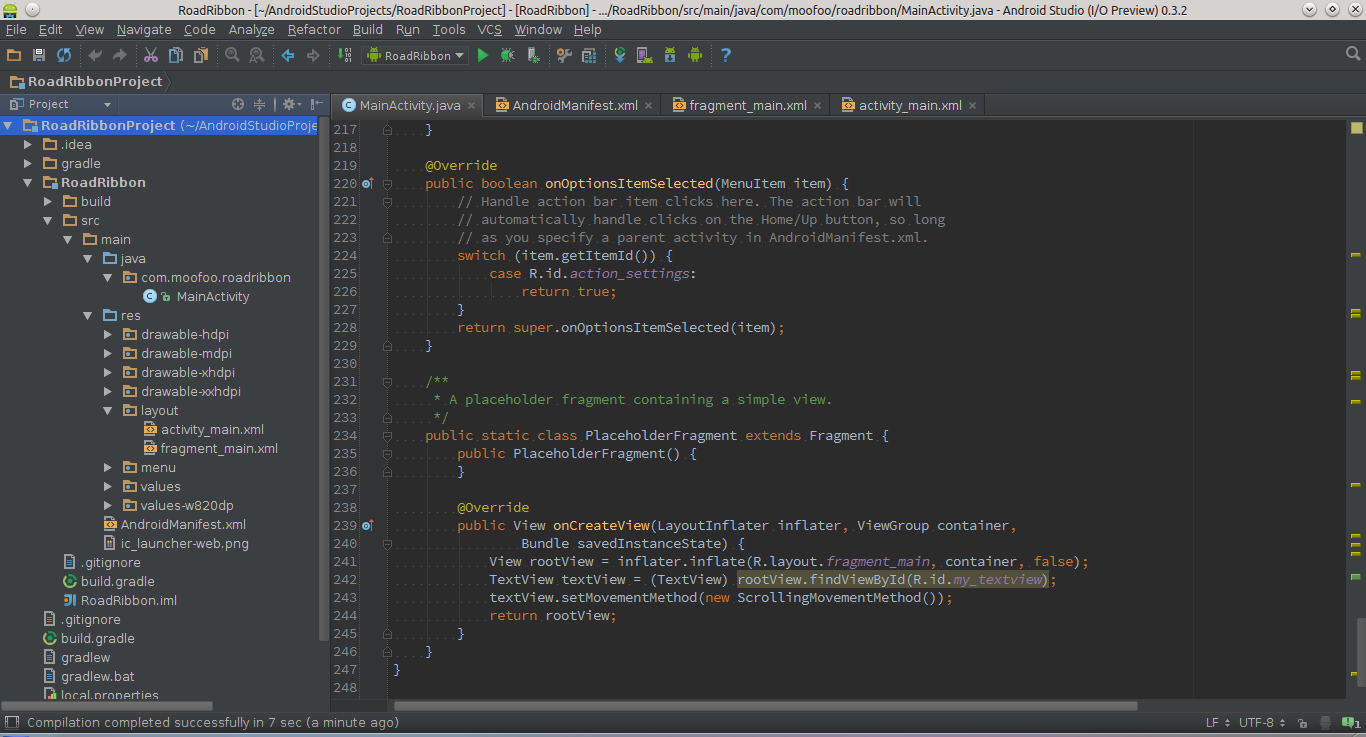
\includegraphics[scale=0.35]{images/android_studio.png}
        	\caption{Середовище розробки AndroidStudio}
        \end{figure}

    \subsection{Загальна схема роботи системи}
    
    Всю схему роботи системи можна поділити на два етапи:
    
    \begin{enumerate}
    	\item \textbf{отримання даних про трек}
    	\item \textbf{візуалізація отриманих даних}
    \end{enumerate}
    
    Отримання даних - це процес подолання певного маршруту, під час якого у пам’яті смартфону відкладаються дані про поточне розташування мобільного агента.
    
    Під час подолання шляху мобільний агент постійно працює в режимі отримання геопозиційних даних від супутників мережі GPS. Тому цей процес є доволі енерго- та ресурсо-ємним для такого не надто потужного пристрою, як смартфон.
    
    Візуалізація даних відбувається на комп’ютері користувача. Уся обробка даних логічно розбита на кілька етапів:
    
    \begin{enumerate}
    	\item \textbf{дешифрація даних, отриманих від мобільних агентів}
    	\item \textbf{підготовка вершинних та індексних даних поверхні}
    	\item \textbf{відображення підготовлених даних у вигляді тривимірної поверхні}
    \end{enumerate}
    
    Дешифрація та підготовка даних до рендерингу - найбільш ресурсоємні процеси. Для дешифрації використовуються регулярні вирази, а для підготовки вершинних даних - повний перебір з використанням деякого математичного апарату. Обидва процеси виконують повний перебір усіх даних, що надійшли від мобільних агентів. Тому це найбільш тривалі у часі задачі.
    
    Відображення підготованих даних навантажує лише графічний процесор комп’ютера користувача. Для оптимізації цієї ділянки проекту було використано \textbf{VBO} - вершинні буфери.

	Нижче наведено діаграму загальної схеми роботи:
	
	\vspace{3em}
	\begin{figure}	
		\centering 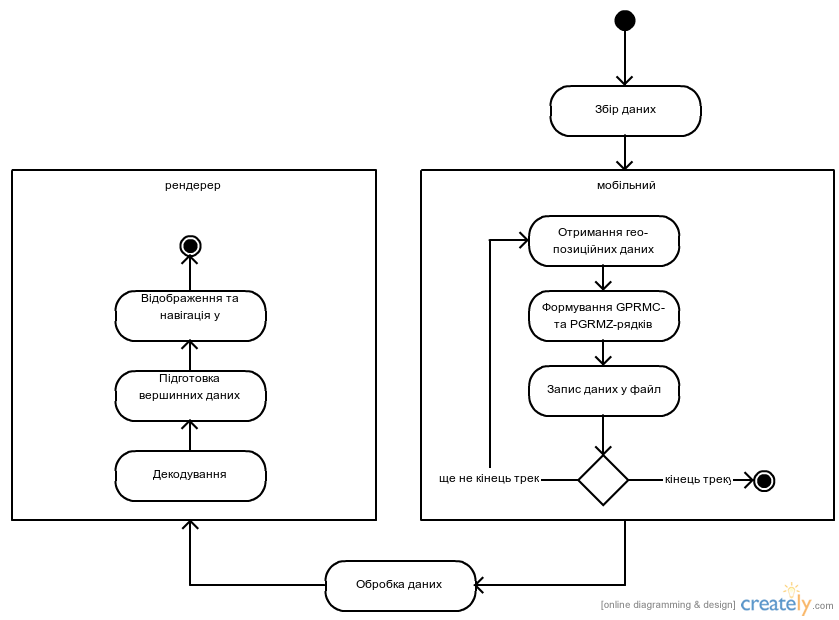
\includegraphics[scale=0.5]{images/general_workflow.png}
		\caption{Загальна схема роботи системи}
	\end{figure}

	\subsection{Архітектура мобільного агента}
	
	Мобільний агент складається з єдиного класу - \textit{MainActivity}. В цьому класі описано логіку завантаження мобільного додатку та основного циклу роботи додатку.
	
	При завантаженні, програма намагається приєднатись до супутників системи GPS та отримати геопозиційні дані. Як тільки їй це вдається, програма переходить в основний режим роботи - постійно зчитує та записує до файлу дані про положення мобільного агенту.
	
	Програма оновлює дані про гео-положення щосекунди. І щосекунди формує з отриманих даних два рядки - \textbf{рядок, що містить широту та довготу} та \textbf{рядок, що містить інформацію про рівень над рівнем моря}. Щоразу, коли рядки сформовано, програма додає їх до файлу на SD-карті пристрою.
	
	\textit{Оновлення файлу} (виконується приблизно щосекунди) - це набір операцій відкриття, запису та закриття файлу з даними. Виконання цих операцій щосекунди пов’язане з можливою помилкою, за якої дескриптор файлу даних залишиться у відкритому стані, якщо програма випадково завершиться. Тому, з метою збереження отриманих даних, відкриття та закриття файлу "обгортають" отримання та обробку даних.
	
	\vspace{2em}
	\begin{figure}
		\centering 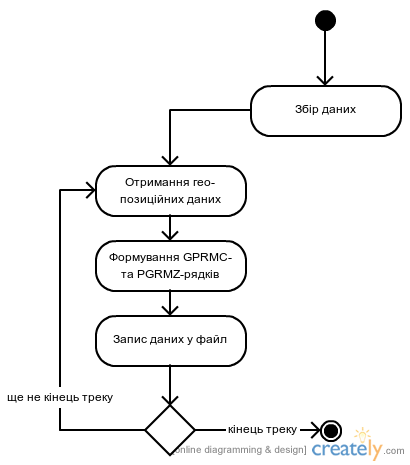
\includegraphics[scale=0.5]{images/mobile_agent_workflow.png}
		\caption{Схема роботи мобільного агента}
	\end{figure}
	
	\vspace{2em}
	\begin{figure}
		\centering 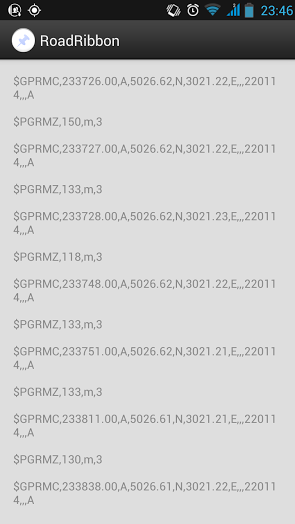
\includegraphics[scale=0.75]{images/mobile_screen.png}
		\caption{Мобільний агент в роботі}
	\end{figure}
        
    \subsection{Алгоритм отримання та збереження гео-даних}
    
    Отримавши дані від GPS-приймача, мобільний агент одразу ж формує з них два рядки:
    
    \begin{enumerate}
    	\item \textbf{рядок GPRMC} - дані про широту та довготу
    	\item \textbf{рядок PGRMZ} - дані про висоту над рівнем моря
    \end{enumerate}
    
	Формується два рядки наступного вигляду:
	
	\begin{lstlisting}
	$GPRMC,113138.00,A,5026.59,N,3021.22,E,,,160114,,,A
	$PGRMZ,195,m,3
	\end{lstlisting}
    
    Збереження відбувається у файл, ім’я якого містить часовий штамп - дату та час початку збору даних мобільним агентом. Це дозволяє сортувати дані ще на етапі міграції даних з мобільного агента на комп’ютер користувача.
    
    Тут слід відмітити, що за стандартом NMEA-0183, широта та довгота записуються у форматі \textbf{DDMM.MM}, де \textbf{DD} - дві цифри градусної міри кута, а \textbf{MM.MM} - хвилини та кількість секунд у вигляді частини хвилини.
    
    Тобто, якщо широта гео-локації рівна $50^\circ 44' 15''$, то у форматі NMEA-0183 ця величина буде рівна $50^\circ; 44' + (\frac{15}{60})' = 50^\circ 44.25'$ і записана як як $5044.25$
    
    Структура мобільного агента мінімальна для зниження ресурсовитрат смартфону. Нижче наведена діаграма класів мобільного агента.
    
    \vspace{3em}
    \begin{figure}
    	\centering 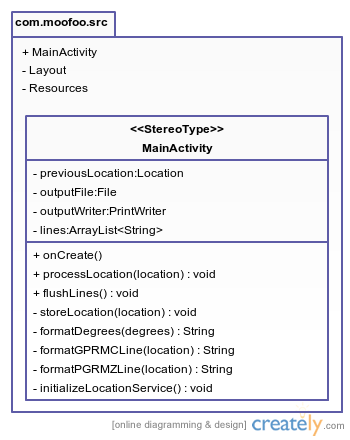
\includegraphics[scale=0.75]{images/mobile_agent_classes.png}
    	\caption{Діаграма класів мобільного агента}
    \end{figure}

    \subsection{Архітектура рендерера}
    
    Рендерер - найбільш ресурсоємна частина системи. Вона складається з кількох класів, кожен з яких несе відповідальну роль в побудові результуючого зображення.
    
    Нижче наведена діаграма діяльності та діаграма класів рендерера:
    
    \vspace{3em}
    \begin{figure}
		\centering 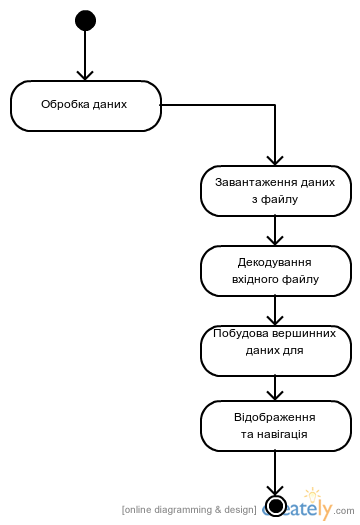
\includegraphics[scale=0.5]{images/renderer_workflow.png}
		\caption{Схема роботи рендерера}
	\end{figure}
	
	\newpage
	\begin{landscape}
		\begin{figure}
			\centering 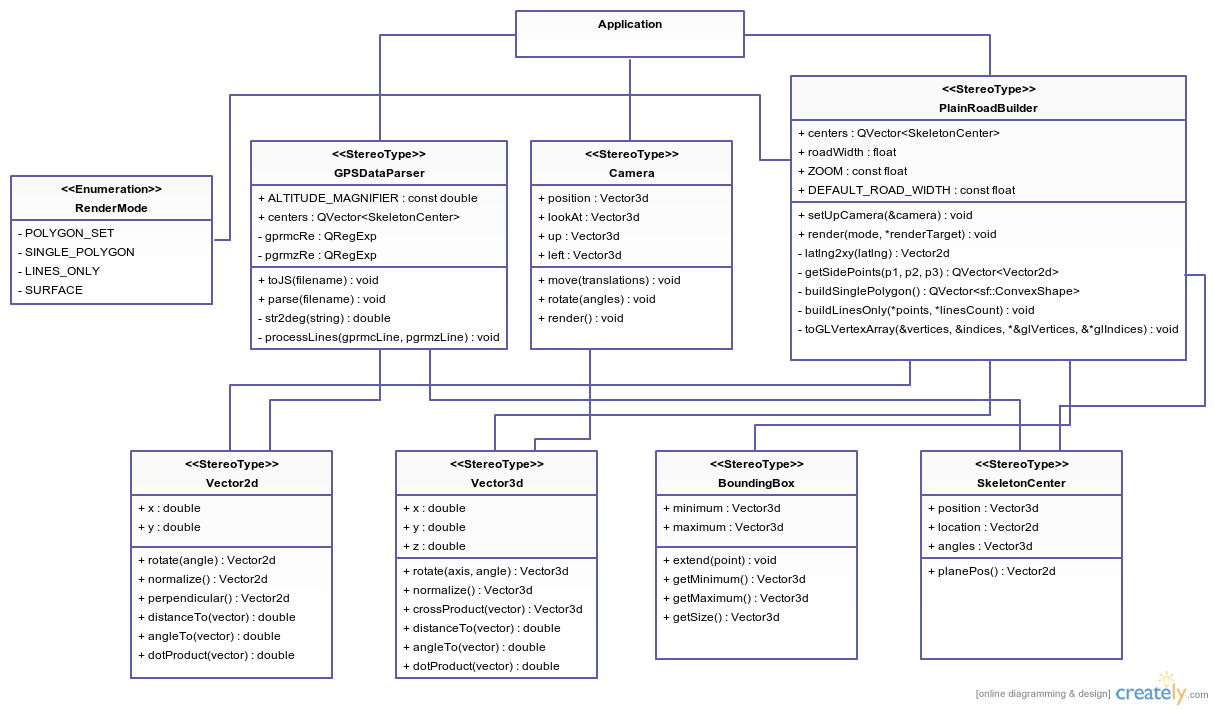
\includegraphics[scale=0.5]{images/renderer_classes.png}
			\caption{Діаграма класів рендерера}
		\end{figure}
	\end{landscape}

	\subsection{Алгоритм завантаження даних}
	
	Формат даних мобільного агента вимагає, аби за кожним рядком, що містить дані про розташування йшов рядок, що містить дані про висоту над рівнем моря у цьому розташуванні. Тому для дешифрування файлу даних створено два регулярних вирази:
	
	\begin{enumerate}
		\item \textbf{gprmcRe} - регулярний вираз для розбору рядка з розташуванням
		\item \textbf{pgrmzRe} - регулярний вираз для розбору рядка з інформацією про висоту над рівнем моря
	\end{enumerate}
	
	З файлу даних в циклі зчитується по два рядки, після чого кожен з них перевіряється на відповідність своєму регулярному виразу. Якщо бодай один з рядків не відповідає шаблону - поточна ітерація пропускається та виводиться відповідне повідомлення про помилку.
	
	Після порівняння з шаблоном, зчитані два рядки розбиваються на відповідні груповані частини тексту, вказані у регулярних виразах. Кожна зі знайдених частин рядка перетворюється у відповідності до інформації, що вона несе в собі. Так, виділяються \textbf{широта}, \textbf{довгота} (перетворені у десятковий формат) та \textbf{висота над рівнем моря}. Усі ці дані заповнюють об’єкт класу \textbf{SkeletonCenter} (\textit{центр кістяка}).
	
	Отриманий набір центральних вузлів передається на метод побудови двовимірного кістяка дороги, або ж тривимірної поверхні треку - в залежності від режиму побудови.
	
	\subsection{Алгоритм побудови двовимірного кістяка дороги}
	
		Отримана послідовність центральних вузлів кістяка очищується від дубльованих центрів. Тобто, з неї викидаються усі центральні вузли, відстань між якими (за формулою відстані між двома векторами \textbf{на площині}, що дає значно більш точні результати, аніж \textit{Great Circle Distance}) менша за порогове значення (\textit{0.01 м}).
		
		Після цього, кожному центральному вузлові кістяка асоціюється пара \textit{бокових} вершин, які утворюють відрізок. Умовою побудови цього відрізка є перпендикулярність лінії, що з’єднує поточний центровий вузел кістяка дороги з наступним та попереднім центровими вузлами. 
		
		Спершу було припущено, що для побудови повороту дороги достатньо семи вершин - по дві пари на кінцях повороту та три вершини на згибі.
		
		\vspace{2em}
		\begin{figure}
			\centering 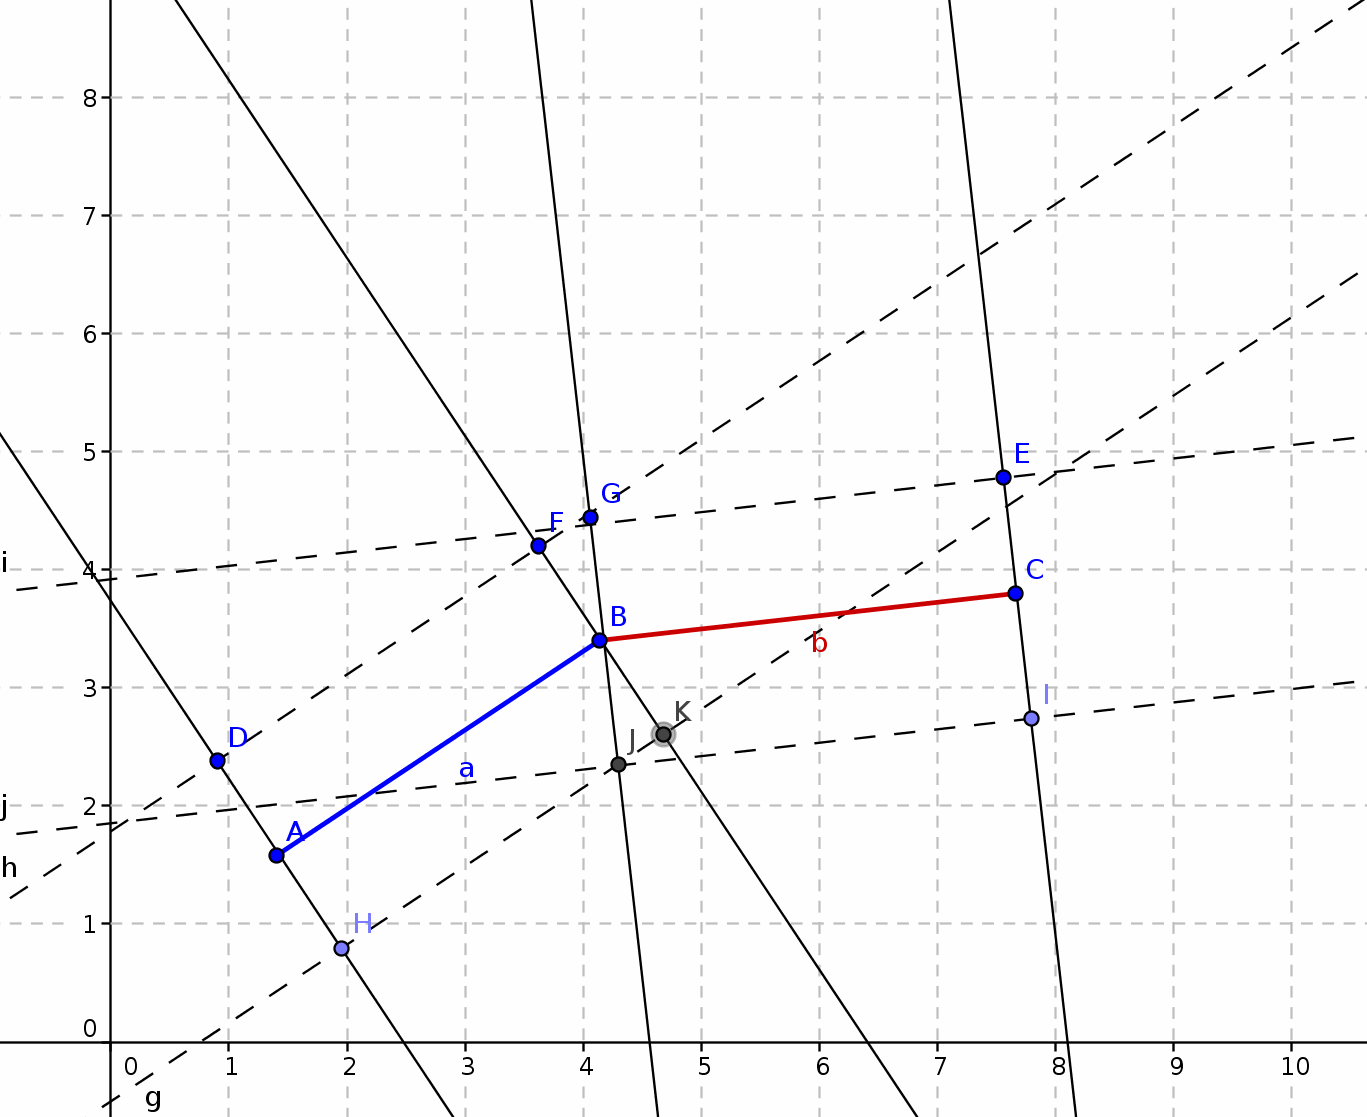
\includegraphics[scale=0.3]{images/perpendicular_2_1.png}
			\caption{Отримання ребер кістяка треку}
		\end{figure}
		
		Так, будується по дві пари вершин - всі лежать на перпендикулярних до "своєї" лінії відрізках, але на різних кінцях. Вони утворюють так звані "бокові точки" ($D, H, F, G, E, I, J, K$). Ці вершини формуватимуть один сегмент тривимірної поверхні треку. Після побудови бокових точок, ті з них, які знаходяться по сторону більшого кута ($\angle ABC$; точки $F$ та $G$) між двома лініями, що з’єднують трійку центральних вузлів ($A, B, C$), залишаються, а дві вершини з протилежного боку кута замінюються однією ($J, K \Rarrow O$).
		
		Обчислюється позиція цієї вершини наступним чином: 
		
		$$
			O = HK \cap IJ
		$$
		
		Але такі обчислення потребують розв’язку системи рівнянь. Що на значних об’ємах даних сильно уповільнює процес побудови кістяка треку.
		
		І в багатьох випадках, коли система має побічні розв’язки, даний алгоритм спрацьовує некоректно. Що і призводить до подібних артефактів:
		
		\vspace{2em}
		\begin{figure}
			\centering 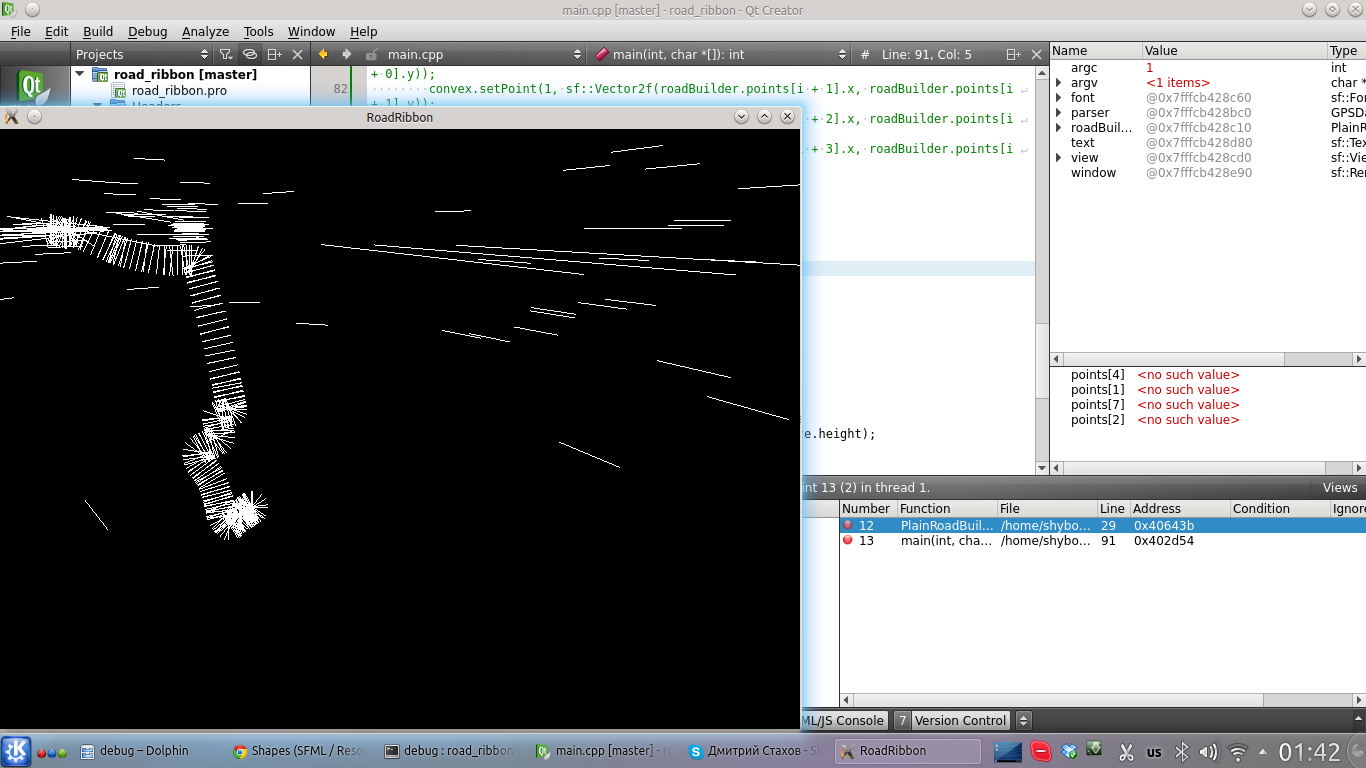
\includegraphics[scale=0.45]{images/road2d_1.png}
			\caption{Артефакти побудови кістяку треку}
		\end{figure}
		
		Тому в решті-решт було вирішено використовувати перпендикуляр до двох ліній, утвориними центровими вузлами кістяка, що суміжні з поточним.
		
		Але оскільки одна лінія не може бути перпендикулярна двом іншим, не паралельним між собою, лініям, то в якості результуючого ребра кістяка обирається такий відрізок, який лежить на бісектрисі кута між перпендикулярами до відрізків, що з’єднують два несуміжні центрові вузли треку.
		
		Якщо, наприклад, потрібно утворити ребро кістяка треку для центрального вузла B (\textit{див. мал.}), тоді потрібно аналізувати попередній до нього у списку центрових вузлів вузол (A) та наступний за ним вузол у списку центрових вузлів (C). Знаходяться два перпендикуляри до прямих, що з’єднують пари центральних вузлів: $c \perp AB$ та $d \perp BC$. Визначається кут між цими перпендикулярами $\alpha = \measuredangle(c, d)$. Визначається градусна міра половини цього кута, $\beta = \frac{\alpha}{2}$ та з точки $B$ відкладається вектор $\overline{a}$, довжина якого рівна половині ширини майбутньої дороги, повернутий на кут $\beta$: $\overline{BF} = \overline{AB} + \overline{a} \circlearrowright \beta$. Аналогічна операція проводиться і для вектора $\overline{BG}$. Таким чином отримується пара вершин $F$ та $G$, які і утворюють ребро для центрового вузла $B$.
		
		\vspace{3em}
		\begin{figure}
			\centering 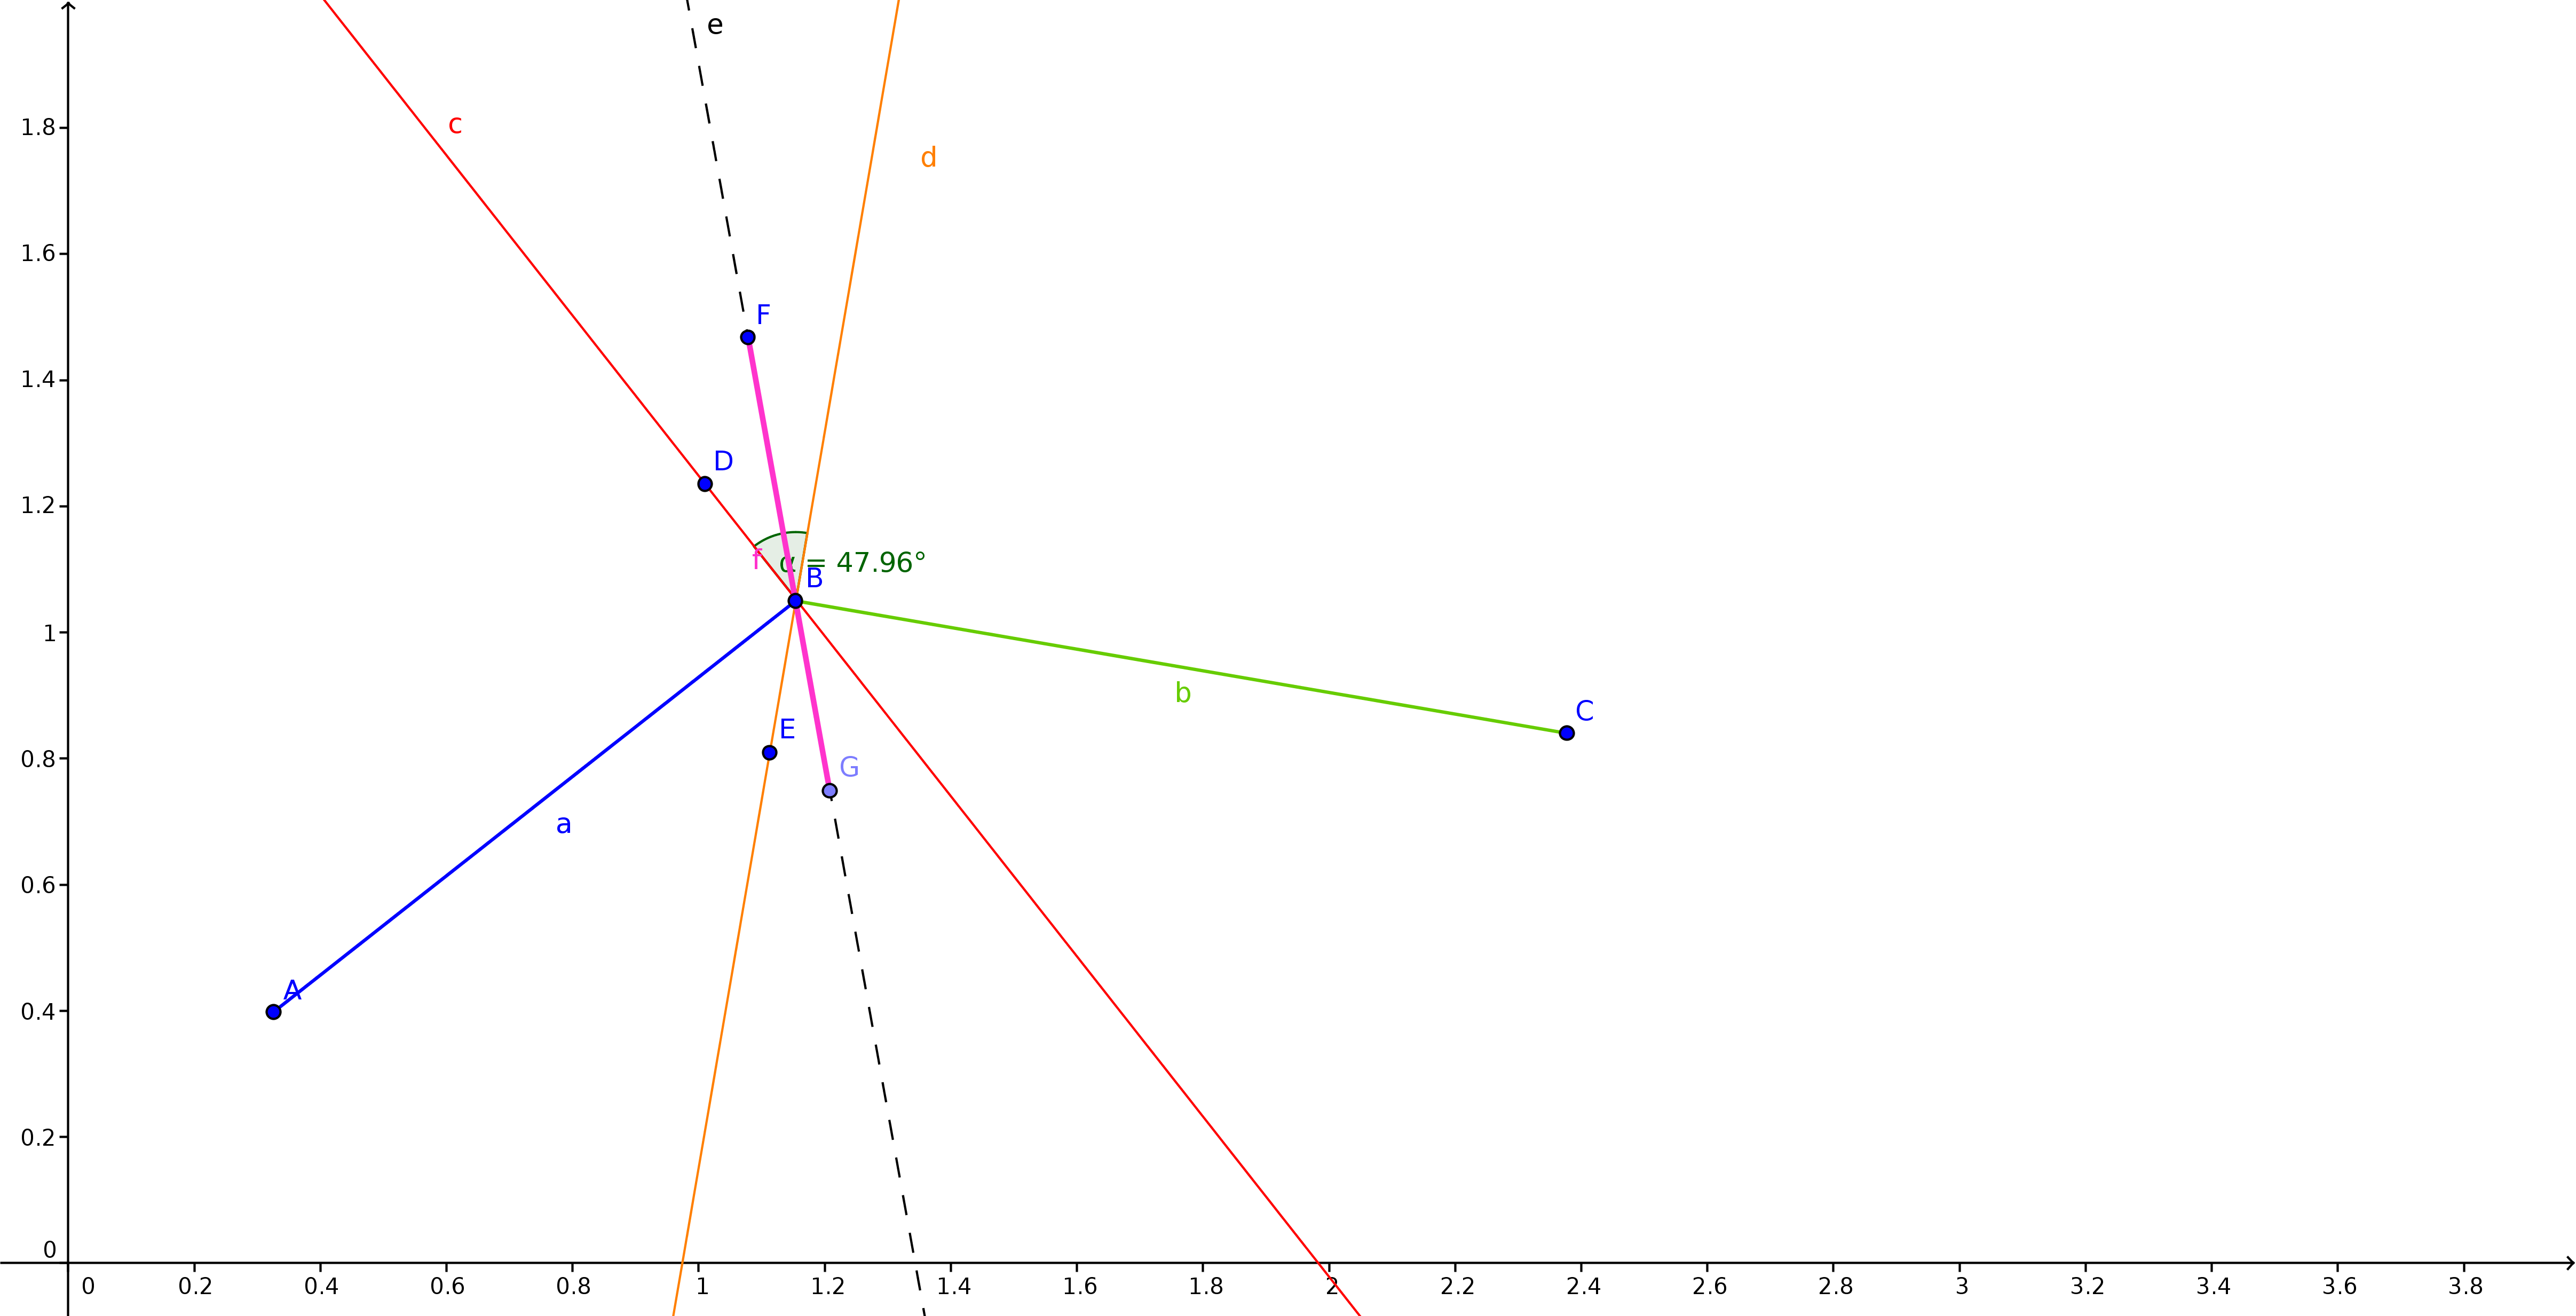
\includegraphics[scale=0.65]{images/perpendicular_1_1.png}
			\caption{Отримання ребер кістяка треку за новим алгоритмом}
		\end{figure}
	
	\subsection{Алгоритм побудови тривимірної поверхні дороги}
	
		Отримана послідовність центральних вузлів кістяка очищується від дубльованих центрів. Тобто, з неї викидаються усі центральні вузли, відстань між якими (за формулою відстані між двома векторами \textbf{у просторі}, що дає значно більш точні результати, аніж \textit{Great Circle Distance}) менша за порогове значення (\textit{0.01 м}).
		
		Всі операції в точності повторюють алгоритм побудови двовимірного кістяка лише з двома поправками:
		
		\begin{enumerate}
			\item \textbf{центрові вузли піднімаються на висоту $h$} - для двовимірного кістяка висота не грала ролі, в той час як для тривимірної поверхні даний критерій є ключовим
			\item \textbf{вершини додаються до списку у заданому порядку} - для подальшого відображення поверхні засобами OpenGL необхідно надати вершини, упорядковані та груповані у чотирикутні сети - впорядковані підмножини з чотирьох елементів, котрі утворять черговий сегмент майбутньої поверхні
		\end{enumerate}
		
		В результаті отримується список, у котрому кожному центровому вузлу відповідає чотири впорядковані вершини - дві з яких утворюють ребро кістяка дороги для попереднього центрового вузла, а дві - для поточного.
	
	\subsection{Навігація у просторі рендерера}
	
		Навігація у просторі створена для більш зручного перегляду отриманої тривимірної поверхні дороги. З цією метою і створений клас \textbf{Camera}. Він цілком відповідає за задання матриці перегляду моделі. Єдина частина рендерера, котра не належить цьому класу але відповідає за зміну перспективи знаходиться в головній функції програми та відповідає за обробку натиснень користувачем клавіш на клавіатурі з метою керування камерою.
		
		Камера являє собою уявну точку (точка огляду, \textbf{eyePos}), з якої ведеться огляд іншої точки (\textbf{lookAt}). Камера обертається довкола точки обертання (\textbf{lookAt}), постійно знаходячись на однаковій відстані від неї. Такий спосіб навігації у віртуальному просторі видався автору найбільш зручним для користувача.
		
		Точку обертання можна переміщувати вздовж треку. Це дає змогу переглянути всю поверхню дороги з усіх боків (враховуючи обертання камери довкола точки огляду). Разом з переміщенням точки обертання, на ідентичну відстань переміщується і точка, з якої якої ведеться спостереження, точка огляду. Це створює приємний ефект переміщення камери.
		
		Точка огляду обертається довкола точки обертання використовуючи таку математичну структуру даних як \textbf{кватерніон}; зокрема - властивість множення кватерніонів.
		
		\vspace{3em}
		\begin{figure}
			\centering 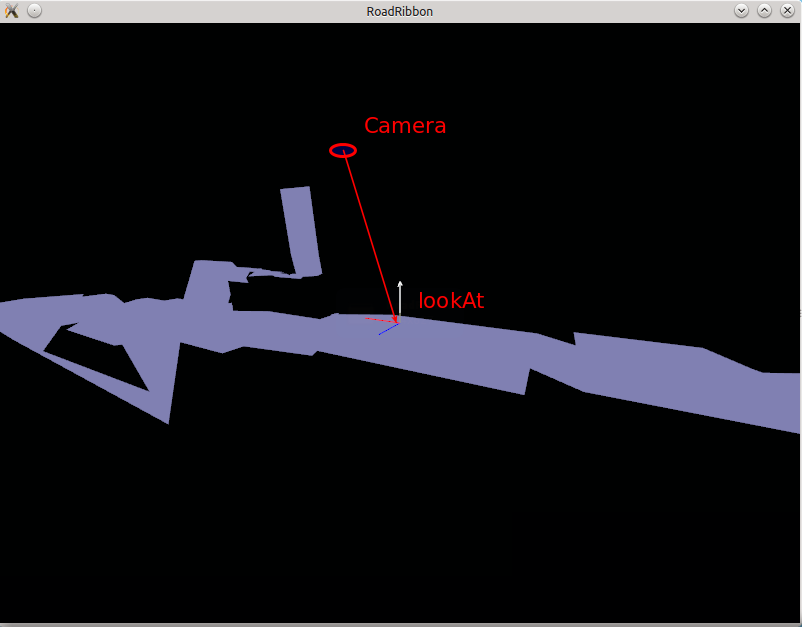
\includegraphics[scale=0.5]{images/camera2.png}
			\caption{Орбітальна камера та точка огляду}
		\end{figure}
       
\clearpage \newpage \section{Функціональний опис архітектури системи}

    \subsection{Модуль мобільного агента}

        \subsubsection{Призначення та короткий опис модуля}

            Даний модуль описує базові математичні структури, що використовуються в програмі в подальшому, та математичні операції над цими структурами. Даний модуль містить базові класи, котрі наслідуються в усіх наступних модулях.

        \subsubsection{Клас MainActivity}
        
        	\textbf{Обробник події створення програми}
        	
        	При створенні програми викликається подія \textit{onCreate}. Її перехоплює та оброблює відповідний метод класу \textbf{MainActivity}. Під час ініціалізації створюється інтерфейс програми та ініціюється процес отримання даних з GPS-приймача. В цей же момент описуються обробники події отримання даних з GPS-приймача.
        	
        	\begin{lstlisting}[language=Java]
@Override
protected void onCreate(Bundle savedInstanceState) {
    super.onCreate(savedInstanceState);

    setContentView(R.layout.activity_main);

    if (savedInstanceState == null) {
        getSupportFragmentManager().beginTransaction()
                .add(R.id.container, 
                	new PlaceholderFragment())
                .commit();
    }

    initializeLocationService();
}
        	\end{lstlisting}
        	
        	\textbf{Обробник події отримання гео-даних}
        	
        	Ця ділянка мобільного агенту перехоплює подію зміни позиції (або ж отримання оновлених даних про позицію).
        	
        	Стиль програмування вимагає максимального розбиття цілісного методу на мінімальні складові з метою подальшої модифікації окремих шматочків системи, а не великого цілого. Тому обробник події зміни позиції просто передає дані про нове положення методу обробки позиції.
        	
\begin{lstlisting}[language=Java]
public void onLocationChanged(Location location) {
	MainActivity.this.processLocation(location);
}
\end{lstlisting}

			Той, в свою чергу, передає керування методу збереження положення \textbf{тоді і лише тоді}, коли нове положення відрізняється від останнього збереженого.
			
\begin{lstlisting}[language=Java]
protected void processLocation(Location location) {
    if ((this.previousLocation != null && 
    	location.distanceTo(this.previousLocation) > 
    		Math.pow(1.0, -3.0)
    	) || (this.previousLocation == null)
   	) {
        this.storeLocation(location);
    }

    this.previousLocation = location;
}
\end{lstlisting}

			Збереження положення поділене на два етапи:
			
			\begin{enumerate}
				\item \textbf{формування двох текстових рядків}, які містять інформацію про положення та висоту над рівнем моря в цій гео-позиції; якщо обидва рядки корректно сформовані - вони додаються до черги на запис у файл
				\item \textbf{запис даних у файл} - відбувається виштовхування всіх накопичених рядків з черги у файл
			\end{enumerate}
			
\begin{lstlisting}[language=Java]
protected void storeLocation(Location location) {
    try {
        String gprmcLine = this.formatGPRMCLine(location);
        String pgrmzLine = this.formatPGRMZLine(location);

        this.lines.add(gprmcLine);
        this.lines.add(pgrmzLine);

        this.addTextMessage(gprmcLine);
        this.addTextMessage(pgrmzLine);

        this.flushLines();
    } catch (Exception e) {
        // ...

        return;
    }
}
\end{lstlisting}
        	
        	\textbf{Метод форматування рядків з даними}
        	
        	Рядки формуються за допомогою можливостей форматування рядків, дат та чисел Java.
        	
\begin{lstlisting}[language=Java]
protected String formatDegrees(double lat) {
    long D = Math.round(lat);
    double m = (lat - D) * 60.0;
    DecimalFormatSymbols otherSymbols = new 
    	DecimalFormatSymbols(Locale.UK);

    String res = String.format("%02d%s",
            D,
            new DecimalFormat("##.##", otherSymbols).format(m)
    );

    return res;
}

protected String formatGPRMCLine(Location location) {
    String lat = this.formatDegrees(location.getLatitude());
    String lng = this.formatDegrees(location.getLongitude());

    Calendar cal = Calendar.getInstance();
    String time = new SimpleDateFormat("HHmmss.00").format(
    	cal.getTime()
    );
    String date = new SimpleDateFormat("ddMMyy").format(
    	cal.getTime()
    );

    return String.format(
            "$GPRMC,%s,A,%s,N,%s,E,,,%s,,,A\r\n",
            time,
            lat,
            lng,
            date
    );
}

protected String formatPGRMZLine(Location location) {
    // $PGRMZ,93,m,3 - altitude
    long alt = Math.round(location.getAltitude());

    return String.format(
            "$PGRMZ,%02d,m,3\r\n",
            alt
    );
}
\end{lstlisting}
        	
        	\textbf{Метод запису даних у файл}
        	
        	Для запису у файл створюється об’єкт класу \textit{File} з іменем, що містить поточну дату та час. Якщо такий файл вже існує - дані будуть додані у кінець цього файлу. Файл створюється в кореневому каталозі SD-карти смартфону.
        	
        	Після відкриття відповідного файлу, дані з черги записуються у файл, а сама черга - очищається.
        	
\begin{lstlisting}[language=Java]
protected void flushLines() {
    try {
        if (this.outputFile == null) {
            Calendar cal = Calendar.getInstance();
            String filename = String.format(
            	"roadribbon_%s.txt",
                new SimpleDateFormat("ddMMyyyy_hhmmss").
                	format(cal.getTime())
            );

            File dir = new File(
            	Environment.getExternalStorageDirectory(), 
            	"/RoadRibbon"
            );
            dir.mkdirs();

            this.outputFile = new File(dir, filename);
        }

        FileOutputStream stream = new FileOutputStream(
        	this.outputFile, true
        );
        this.outputWriter = new PrintWriter(stream);

        for (String line : this.lines) {
            this.outputWriter.print(line);
        }

        this.outputWriter.close();

        this.lines.clear();
    } catch (Exception e) {
        // ...

        return;
    }
}
\end{lstlisting}
        
     \subsection{Модуль рендерера}
     
     	\subsubsection{Клас Vector2d}
     	
     		Даний клас описує вектор на площині та деякі операції над векторами на площині, як, наприклад, \textit{поворот}, \textit{визначення кута між двома векторами}, \textit{визначення вектору}, \textit{перпендикулярного до даного}, \textit{нормалізація вектора}, тощо.
     	
        	\textbf{Конструктор класу}

            \begin{lstlisting}[language=C++]
            Vector2d(_x = 0.0, _y = 0.0);
            \end{lstlisting}

            По замовчуванню всі координати вектора задані нульовими, тож можливий варіант виклику конструктора:

            \begin{lstlisting}
            new Vector2d(); 
            \end{lstlisting}     	
     	
	     	\textbf{Визначення вектора-перпендикуляра}
	     	
	     	Якщо дано вектор, $\overline{a} (x_1, y_1)$ тоді вектор $\overline{b} (x_2, y_2) \perp \overline{a}$ якщо $\overline{a} \cdot \overline{b} = 0$.
	     	
	     	Для того, щоб знайти координати перпендикулярного вектора необхідно розв’язати два рівняння:
	     	
	     	$$
	     		\overline{b}(x_2, y_2) \perp \overline{a}(x_1, y_1) \Rightarrow (x_1 \cdot x_2) + (y_1 \cdot y_2) = 0;
	     	$$
	     	
			Припустимо, що $x_2 = 1$. Тоді:
	     	
	     	$$
	     		x_1 + y_1 \cdot y_2 = 0 \Rightarrow y_2 = -\frac{x_1}{y_1}
	     	$$
	     	
	     	Так само знаходиться й $x_2$:
	     	
	     	$$
	     		y_2 = 1 \Rightarrow x_1 \cdot x_2 + y_1 = 0 \Rightarrow x_2 = -\frac{y_1}{x_1}
	     	$$
	     	
\begin{small}
\begin{lstlisting}[language=C++]
Vector2d Vector2d::perpendicular()
{
    if (this->y != 0.0)
    {
        return Vector2d(1.0, -this->x / this->y);
    } else if (this->x != 0.0)
    {
        return Vector2d(-this->y / this->x, 1.0);
    } else
    {
        return Vector2d(0, 0);
    }
}
\end{lstlisting}
\end{small}
	     	
	    \textbf{Обертання вектора}
	    
	    Вектор можна обернути довкола його початку за допомогою тригонометричних функцій.
	    
\begin{small}
\begin{lstlisting}[language=C++]
Vector2d Vector2d::rotate(double angle)
{
    return Vector2d(
        (this->x * cos(angle)) - (this->y * sin(angle)),
        (this->x * sin(angle)) + (this->y * cos(angle))
    );
}
\end{lstlisting}
\end{small}
     	
    	\subsubsection{Клас Vector3d}

            Даний клас описує вектор у просторі та деякі операції над векторами.

            \textbf{Конструктор класу}

            \begin{lstlisting}[language=C++]
            Vector3d(_x = 0.0, _y = 0.0, _z = 0.0);
            \end{lstlisting}

            По замовчуванню всі координати вектора задані нульовими, тож можливий варіант виклику конструктора:

            \begin{lstlisting}
            new Vector3d(); 
            \end{lstlisting}

            \textbf{Операції над векторами}

            Даний клас описує більшість необхідних операцій над векторами, як-то: множення та ділення на скаляр та на вектор, додавання та віднімання. Також описані додаткові мктоди: визначення модуля вектора (\textit{\textbf{length}}), порівняння рівності та нерівності векторів (\textit{\textbf{==}}, \textit{\textbf{!=}}), визначення кута між двома векторами (\textit{\textbf{angle\_to(vector)}}), поворот навколо заданої осі на заданий кут (\textit{\textbf{rotate(angle, axis)}}).

            Визначення кута між двома векторами реалізовано за допомогою формули скалярного добутку векторів:

            $$ \phi = \arccos \frac{\vec{a}\vec{b}}{\abs{\vec{a}}\abs{\vec{b}}} $$

            Поворот вектора навколо заданої осі на заданий кут реалізовано за допомогою розгорнутої форми множення кватерніонів:


            Нехай $\vec{u}$ - вектор-вісь, навколо якої обертатимемо вектор; $\vec{v}$ - вектор, котрий обертатимемо, а $\alpha$ - кут, на який обертатимемо $\vec{v}$ навколо вісі $\vec{u}$.

            Якщо кватерніон $ q = \cos \frac{\alpha}{2} + \vec{u} \sin \frac{\alpha}{2} $, то

            $$ \vec{v'} = q \vec{v} q^{-1} = \left( \cos \frac{\alpha}{2} + \vec{u} \sin \frac{\alpha}{2} \right) \, \vec{v} \, \left( \cos \frac{\alpha}{2} - \vec{u} \sin \frac{\alpha}{2} \right) $$

            або

            \begin{displaymath}
                \begin{array}{lll}
                    \vec{v'} &=& \vec{v} \cos^2 \frac{\alpha}{2} + (\vec{u}\vec{v} - \vec{v}\vec{u}) \sin \frac{\alpha}{2} \cos \frac{\alpha}{2} - \vec{u}\vec{v}\vec{u} \sin^2 \frac{\alpha}{2} \\
                    &=& \vec{v} \cos^2 \frac{\alpha}{2} + 2 (\vec{u} \times \vec{v}) \sin \frac{\alpha}{2} \cos \frac{\alpha}{2} - (\vec{v} (\vec{u} \cdot \vec{u}) - 2 \vec{u} (\vec{u} \cdot \vec{v})) \sin^2 \frac{\alpha}{2} \\
                    &=& \vec{v} (\cos^2 \frac{\alpha}{2} - \sin^2 \frac{\alpha}{2}) + (\vec{u} \times \vec{v}) (2 \sin \frac{\alpha}{2} \cos \frac{\alpha}{2}) + \vec{u} (\vec{u} \cdot \vec{v}) (2 \sin^2 \frac{\alpha}{2}) \\
                    &=& \vec{v} \cos \alpha + (\vec{u} \times \vec{v}) \sin \alpha + \vec{u} (\vec{u} \cdot \vec{v}) (1 - \cos \alpha) \\
                    &=& (\vec{v} - \vec{u} (\vec{u} \cdot \vec{v})) \cos \alpha + (\vec{u} \times \vec{v}) \sin \alpha + \vec{u} (\vec{u} \cdot \vec{v})
                \end{array}
            \end{displaymath}
            
\begin{small}
\begin{lstlisting}[language=C++]
Vector3d Vector3d::rotate(Vector3d axis, double radianAngle)
{
    Vector3d v = *this, u = axis;

    return ((v - (u * (u.dotProduct(v)))) * cos(radianAngle)) +
            (u.crossProduct(v) * sin(radianAngle)) +
            (u * (u.dotProduct(v)));
}
\end{lstlisting}
\end{small}

        \subsubsection{Клас GPSDataParser}
        
        \textbf{Короткий опис класу}
        
        Даний клас призначений для зчитування та дешифрування даних, отриманих в результаті роботи мобільних агентів під час подолання ними певних маршрутів.
        
        Клас дає змогу перетворити файл з даними або у скрипт мовою програмування \textbf{JavaScript}, який можна використати для перегляду пройденого мобільним агентом маршруту на мапі (за допомогою наявної HTML-сторінки в директорії \textbf{test}), або у набір центрових вузлів маршруту.
        
        \textbf{Конструктор}
        
        В конструкторі об’єкту класу \textbf{GPSDataParser} створюється два регулярних вирази - по одному на кожен з рядків, які "розуміє" рендерер:
        
\begin{small}
\begin{lstlisting}[language=C++]
void GPSDataParser::init()
{
gprmcRe = QRegExp("\\$GPRMC,((\\d\\d)(\\d\\d)(\\d+\\.\\d+)),([A-Z])...");

pgrmzRe = QRegExp("\\$PGRMZ,(\\d+),(m|f),(\\d+)");

centers.clear();
}
\end{lstlisting}
\end{small}
        
        \textbf{Конвертація у JS-файл}
        
        При конвертації у JavaScript-файл (з метою подальшого використання у HTML-сторінці, на якій відображається мапа з пройденим мобільним агентом маршрутом) створюється файл, котрий задає об’єкту \textbf{window} поле \textbf{waypoints} - масив пар координат, що відповідають конкретному центровому вузлу кістяка маршруту.

\begin{small}        
\begin{lstlisting}[language=C++]
void GPSDataParser::toJS(QString filename)
{
    if (centers.size() < 1)
    {
        return;
    }

    QFile f(filename);

    f.open(QIODevice::WriteOnly | QIODevice::Text);

    QTextStream out(&f);

    out << "window.waypoints = [\n";

    for (long long i = 0; i < centers.size(); i++)
    {
        QString line = QString("[ %1, %2 ]").
        	arg(centers[i].location.x).
        	arg(centers[i].location.y);

        out << line;

        if (i < centers.size() - 1)
        {
            out << ",";
        }

        out << "\n";
    }

    out << "];";

    f.close();
}
\end{lstlisting}
\end{small}

		\textbf{Методи обробки рядку гео-позиції}
		
		Методи використовують створені у конструкторі регулярні вирази та зчитані з файлу даних рядки.
		
\begin{small}
\begin{lstlisting}[language=C++]
double GPSDataParser::str2deg(QString str)
{
    QRegExp lat_re("(\\d\\d)(\\d\\d\\.\\d+)"),
            lng_re("(\\d\\d\\d)(\\d\\d\\.\\d+)");

    double degrees = 0.0, minutes_part = 0.0;

    if (lat_re.indexIn(str) != -1)
    {
        degrees = lat_re.cap(1).toDouble();
        minutes_part = lat_re.cap(2).toDouble();

        return degrees + (minutes_part / 60.0);
    } else if (lng_re.indexIn(str) != -1)
    {
        degrees = lng_re.cap(1).toDouble();
        minutes_part = lng_re.cap(2).toDouble();

        return degrees + (minutes_part / 60.0);
    } else
    {
        return 0.0;
    }
}

void GPSDataParser::processLines(QString gprmcLine, QString pgrmzLine)
{
    if (gprmcRe.indexIn(gprmcLine) < 0)
    {
        return;
    }

    if (pgrmzRe.indexIn(pgrmzLine) < 0)
    {
        return;
    }

    Vector2d location = processGPRMCLine(gprmcLine);
    double alt = processPGRMZLine(pgrmzLine) * ALTITUDE_MAGNIFIER;
    Vector3d position = Vector3d(location.x, alt, location.y);

    // TODO: refactor
    SkeletonCenter center(location, position, Vector3d(0, 0, 0));

    centers.push_back(center);
}

Vector2d GPSDataParser::processGPRMCLine(QString line)
{
    gprmcRe.indexIn(line);

    double lat = str2deg(gprmcRe.cap(6)),
           lng = str2deg(gprmcRe.cap(10));

    return Vector2d(lat, lng);
}

double GPSDataParser::processPGRMZLine(QString line)
{
    pgrmzRe.indexIn(line);

    return pgrmzRe.cap(1).toDouble();
}
\end{lstlisting}
\end{small}

        \subsubsection{Клас PlainRoadBuilder}
        
        \textbf{Которкий опис класу}
        
        Даний клас використовується для приведення послідовності центрових вузлів кістяка маршруту до вигляду, зручного для використання бібліотекою OpenGL.
        
        \textbf{Конструктор класу}
        
        В конструкторі послідовність центральних вузлів фільтрується з метою прибрати ідентичні центри, а також кожному центру задається позиція в координатах простору.
        
\begin{small}
\begin{lstlisting}[language=C++]
PlainRoadBuilder::PlainRoadBuilder(QVector<SkeletonCenter> _centers, 
	float roadWidth
)
{
    if (_centers.size() < 3)
    {
        return;
    }

    Vector2d origin = this->latlng2xy(_centers[0].location);

    for (int i = 1; i < _centers.size(); i++)
    {
        while ((i < _centers.size() - 1) && 
        	(_centers[i + 1].location == _centers[i].location)
        ) i++;

        SkeletonCenter center = _centers[i];

        Vector2d xy = this->latlng2xy(centers[i].location, 
        	origin
        );

        center.position = Vector3d(xy.x, 
        	centers[i].position.y * (ZOOM * 4), 
        	xy.y
       	);

        this->centers.push_back(center);
    }

    this->roadWidth = roadWidth;
}
\end{lstlisting}
\end{small}
        
        \textbf{Перетворення широти та довготи в координати у просторі}
        
        \textbf{Побудова вершинних даних}
        
        Для побудови вершинних даних використовуються дані про ребро, що асоційоване з попереднім до поточного оброблюваного центрового вузла дороги.
        
\begin{small}
\begin{lstlisting}[language=C++]
void PlainRoadBuilder::buildPolygonSet(
	QVector<Vector3d>* vertices, QVector<int>* indices
)
{
    for (int i = 1; i < this->centers.size() - 1; i++)
    {
        Vector2d A = this->centers[i - 1].planePos(),
                B = this->centers[i].planePos(),
                C = this->centers[i + 1].planePos(),
                BA = A - B;

        double angle = 0; // M_PI / 16.0;

        if (fabs((C - B).angleTo(A - B) - M_PI) < pow(10.0, -5.0))
        {
            angle = 0;
        }

        Vector2d a = BA.perpendicular().
        			normalize().
        			rotate(angle) * this->roadWidth,
                AL = A + a,
                AR = A - a;

        Vector3d AL3D = 
        	Vector3d(AL.x, this->centers[i].position.y, AL.y),
                AR3D = 
            Vector3d(AR.x, this->centers[i].position.y, AR.y);

        int index = vertices->size();

        if (i == 1)
        {
            vertices->push_back(AL3D);
            vertices->push_back(AR3D);
        } else
        {
            vertices->push_back(AR3D);
            vertices->push_back(AL3D);
            vertices->push_back(AL3D);
            vertices->push_back(AR3D);

            indices->push_back(index - 2);
            indices->push_back(index - 1);
            indices->push_back(index + 0);
            indices->push_back(index + 1);
        }
    }

    {
        Vector2d A = this->centers[this->centers.size() - 1].
        	planePos(),
                B = this->centers[this->centers.size() - 2].
            planePos(),
                BA = A - B,
                a = BA.perpendicular().
                	normalize().
                	rotate(M_PI / 16.0) * this->roadWidth,
                AL = A + a,
                AR = A - a;

        Vector3d AL3D = 
        	Vector3d(AL.x, 
        		this->centers[this->centers.size() - 1].
	        		position.y, 
        		AL.y
        	);
        		
        Vector3d AR3D = 
            Vector3d(AR.x, 
            	this->centers[this->centers.size() - 1].
            		position.y, 
            	AR.y
            );

        vertices->push_back(AL3D);
        vertices->push_back(AR3D);
    }
}
\end{lstlisting}
\end{small}

        \subsubsection{Клас Camera}
        
        \textbf{Короткий опис класу}
        
        Даний клас застосовується для перетворень матриці \textit{GL\_MODELVIEW}.
        
        \textbf{Конструктор}
        
        У конструкторі задаються значення "по замовчуванню" для вектору напрямку догори та для вектору напрямку ліворуч від камери.
        
\begin{small}
\begin{lstlisting}[language=C++]
Camera::Camera(Vector3d _position, Vector3d _lookAt)
{
    this->position = _position;
    this->lookAt = _lookAt;
    this->up = Vector3d(0, 1, 0);
    this->left = Vector3d(1, 0, 0);
}
\end{lstlisting}
\end{small}
        
        \textbf{Переміщення камери}
        
        Операція переміщення здійснює зміщення вектору \textbf{eyePos} та \textbf{lookAt} на однакову величину (на однаковий вектор).
        
\begin{small}
\begin{lstlisting}[language=C++]
void Camera::move(Vector3d translate)
{
    Vector3d v1 = this->position;
    v1.y = this->lookAt.y;

    Vector3d tz = (this->lookAt - v1).normalize() * -translate.z;
    Vector3d ty = Vector3d(0, 1, 0) * translate.y;

    Vector3d delta = tz + ty;

    this->position += delta;
    this->lookAt += delta;
}
\end{lstlisting}
\end{small}
        
        \textbf{Обертання камери}
        
        Камера обертається довкола точки \textbf{lookAt}. Для цього, виконується два повороти:
	
		\begin{enumerate}
			\item \textbf{горизонтальний поворот} - поворот довкола осі $OY$
			\item \textbf{вертикальний поворот} - поворот довкола осі $OX$
		\end{enumerate}
        
        Для горизонтального повороту, вектор $\overline{lookAt - eyePos}$ за допомогою властивостей операції множенняя кватерніонів (у розгорнутому вигляді) повертається на кут $\alpha_y$ довкола вектора \textbf{up}. Потім вектор \textbf{left} повертається довкола вектора \textbf{up} на такий самий кут.
        
        Для вертикального повороту, спершу вектор \textbf{up} повертається довкола вектора \textbf{left} на заданий кут, після чого вектор $\overline{lookAt - eyePos}$ повертається на такий самий кут довкола вектора \textbf{left}. 
        
\begin{small}
\begin{lstlisting}[language=C++]
void Camera::rotate(Vector3d angles)
{
    this->position = (this->position - this->lookAt).
    	rotate(this->up, angles.y) + this->lookAt;
    this->left = this->left.rotate(this->up, angles.y);

    this->position = (this->position - this->lookAt).
    	rotate(this->left, angles.x) + this->lookAt;
}
\end{lstlisting}
\end{small}

	\subsubsection{Клас BoundingBox}
        
        \textbf{Короткий опис класу}
        
        Даний клас застосовується для визначення прямокутника мінімального розміру, необхідного аби вмістити множину точок.
        
        \textbf{Конструктор}
        
        Під час створення об’єкту класу \textbf{BoundingBox}, створюються два нульових вектори - \textbf{minBound} та \textbf{maxBound}.
        
        \textbf{Розширення кордонів BoundingBox}
        
        Навіть одна точка може змінити розміри BoundingBox. Якщо бодай одна з координат цієї точки менша за відповідну координату \textbf{minBound} - вектор мінімальної границі прямокутника змінить відповідну координату на значення, задане точкою. Те ж вірно в зворотньому порядку і для вектору максимальної границі прямокутника, координати якого зміняться якщо вони менші за відповідні координати заданої точки.
        
\begin{small}
\begin{lstlisting}[language=C++]
void BoundingBox::extend(Vector2d point)
{
    if (point.x < minimumBound.x)
        minimumBound.x = point.x;

    if (point.y < minimumBound.y)
        minimumBound.y = point.y;

    if (point.x > maximumBound.x)
        maximumBound.x = point.x;

    if (point.y > maximumBound.y)
        maximumBound.y = point.y;
}
\end{lstlisting}
\end{small}
        
    \clearpage \newpage 
    
    \section{Застосування системи в реальному житті}

	\subsection{Апробація в межах короткого маршруту}
	
	В межах короткого маршруту в м. Києві, показаного на мапі, система проявила себе доволі непогано. Як і передбачалось, в підземних переходах та у місцях, густо заставлених будівлями, сигнал від супутників приходить спотворений та/або із затримками, чим і спричинені візуальні артефакти на тривимірній поверхні пройденого шляху.
	
	При швидкому переміщенні у міському автобусі похибки були значно меншими внаслідок меншої густоти об’єктів вздовж дороги та більш плавному пересуванню транспортного засобу та смартфону всередині нього.
	
	Розмір файлу з даними мобільного агента за \textbf{15 хв} роботи програми не перевищив \textbf{40 кБ}.
	
		\begin{figure}
			\centering 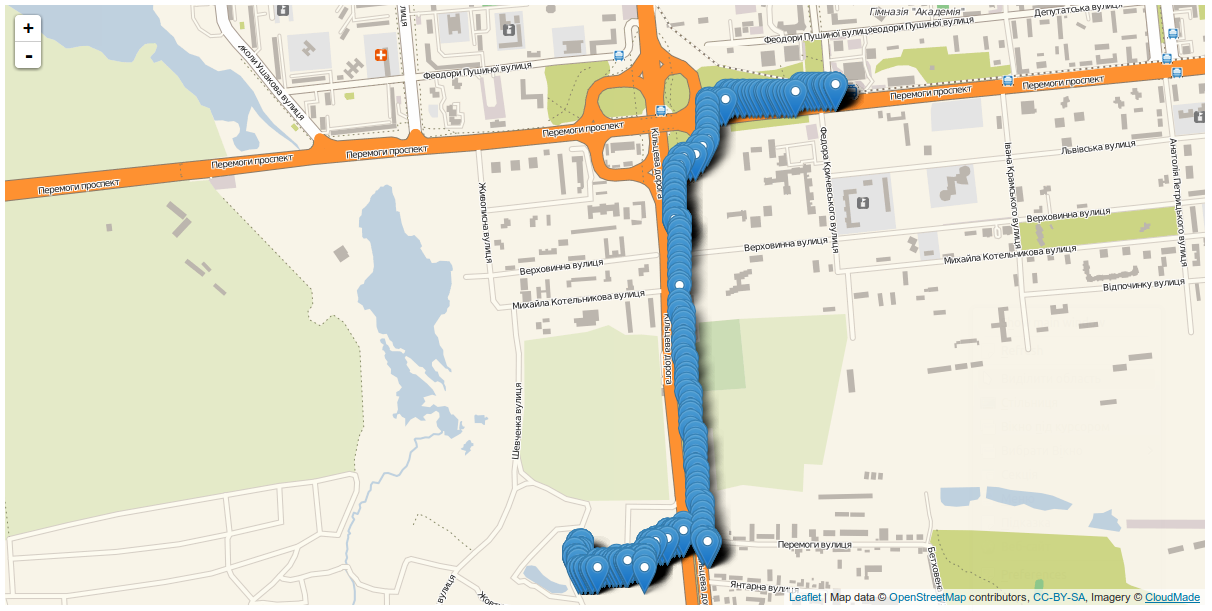
\includegraphics[scale=0.35]{images/results1.png}
			\vspace{2em}
			\centering 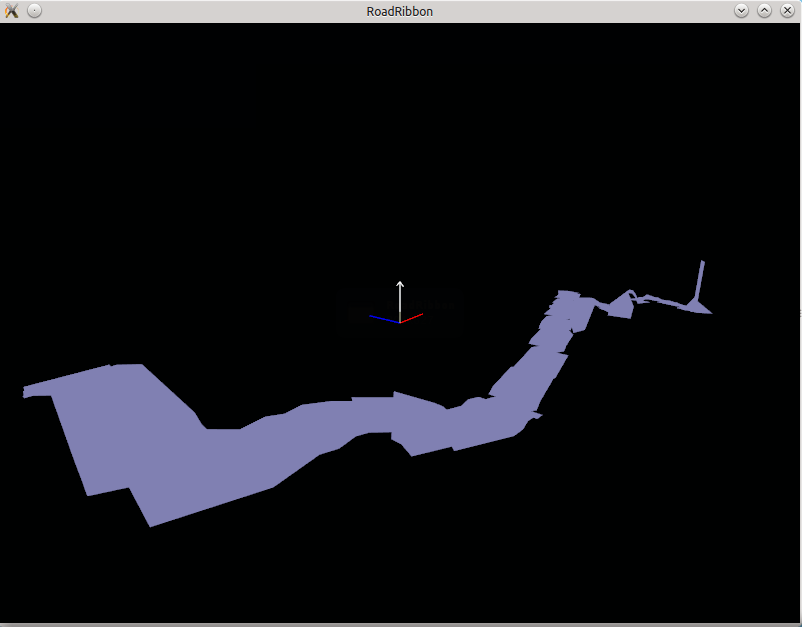
\includegraphics[scale=0.5]{images/results2.png}
			\caption{Візуалізація пройденого треку на мапі та у рендерері}
		\end{figure}

  \clearpage \newpage
  
  \section*{Висновки}
  \addcontentsline{toc}{section}{Висновки}

    Під час виконання роботи було проаналізовано існуючі системи та формати відстеження гео-позиції на планеті та висоти над рівнем моря у цій позиції за допомогою супутників мережі GPS.

    В рамках роботи було створено систему для відслідковування зміни гео-положення та запису пройденого маршруту у файл на смартфоні та систему візуалізації отриманих даних у вигляді тривимірної поверхні пройденого треку. Розроблені модулі показують сильні сторони мов програмування Java та C++, можливості платформ розробки Qt та Android, демонструють функціональну широту бібліотек SFML та OpenGL. Програмний код відповідає сучасним вимогам кодування та простий для розуміння.

    Розроблена система відкриває нові площини для досліджень. Показані ідеї можуть та будуть втілені в інших розробках в галузі гео-кодування та автомобільно-дорожніх системах, системах навігації та гео-інформаційних системах.

\newpage

\bibliographystyle{gost2008}
\renewcommand\bibname{Використана література}
\bibliography{literature.bib}

\end{document}
